% ----------------------------------------------------------
\chapter{Experiments, Results and Discussion} \label{cap:proposal}

% Falar que os experimentos foram divididos em três conforme as perguntas. 
% Os experimentos não foram descritos na ordem que foram executados mas numa ordem conforme as perguntas.
% As bases de dados foram aumentando conforme os experimentos
% Descrever brevemente os experimentos

In this chapter, we describe the steps followed to answer the research question and its three parts.\footnote{This chapter is adapted from the papers \textcite{Sabo2019},  \textcite{DalPont2020}, and \textcite{Sabo2021}, with substantial degree of overlap.
Some sections from those papers are identical to parts of this dissertation, and others are substantially the same as parts, but in different words. To avoid over-quoting, we offer this note as a general citation and do not provide further citations to these articles in the body of the chapter.}
%
The questions are answered based on three distinct experiments, regarding text representation, text classification and text regression, detailed in Section \ref{sec:text_representation}, \ref{sec:text_classification}, and \ref{sec:text_regression}, respectively. 

The datasets used in each section consider the same type of data, that is, legal judgments from the \gls{JEC} at \gls{UFSC}. Those judgments involve failures on air transport services. However, the amount of data in each section changes as we run the experiments and performed the data collections at \gls{JEC}, during the last two years.

% 
% ----------------------------------------------------------

%----------------------------------------------------------
%
% Describe the order of the experiments
%----------------------------------------------------------
\section{Dataset Construction} \label{sec:dataset_construction}

\subsection{Labeled Dataset from Special Civel Court}
% JEC Dataset


% Retirado da parte de classificação. Adaptar aqui
%A base de dados de treinamento contou com um total de 665 documentos de sentenças, abrangendo as quatro classes. Entretanto, algumas destas sentenças apresentaram mais de um resultado, ou seja, contêm mais de uma classe. Nesses casos, as sentenças foram replicadas para cada uma das classes indicadas em seu dispositivo, resultando em um total de 673 sentenças para o treinamento. Assim, para a classe “procedente”, foram incluídas 214 sentenças; para classe “improcedente”, 70 sentenças; para classe “parcialmente procedente”, 379 sentenças; e para a classe “extinção”, 10 sentenças.

% Cases' result = label in this work

\subsection{Unlabeled Dataset from Brazilian Higher Courts}
% STF, STJ, TJ-SC Dataset

% Warning!! Copy/Paste 
Concerning embeddings training, the first step is to obtain the collection of legal documents from the court web portals, followed by raw text extraction from these documents. To enable us to evaluate the specificity influence of these legal corpora, we divided it into two contexts: related to general legal texts and related to air transport services text.

% Warning!! Copy/Paste
We also collected texts from other general topics (not related to legal domains) that are already compiled and freely available. Having the corpora for legal and miscellaneous contexts, we applied some processing steps to remove noise from texts. To evaluate the influence of corpus size in embeddings training, we divided these three corpora into smaller pieces based on word count.

% Warning!! Copy/Paste 
To train the embeddings it is required large text corpora to be able to get good embeddings. However, in the Brazilian Portuguese language, we could not find any dataset available on the Internet containing enough legal text corpora for our purposes. Thus, we had to build our legal corpora.

% Warning!! Copy/Paste 
Our main sources of legal text are Brazilian courts platforms. We collected judgments from the webpages of Federal Supreme Court (STF), Superior Court of Justice (STJ) and State Court of Santa Catarina (TJ-SC) \cite{STF2020, STJ2020, TJSC2020}. 
We also collected judgments from the JusBrasil portal containing processes related only to failures on air transport service from all State Courts (TJ) from Brazil \cite{Jusbrasil2020}.

% Warning!! Copy/Paste 
Table \ref{tab:count_process} shows the number of processes acquired and word count for each Tribunal:

\begin{table}[htb]
\caption{Acquired process from Courts for Embeddings Training}
\label{tab:count_process}
\centering
\begin{tabular}{@{}crrrr@{}}
\toprule
\textbf{Source}      & \multicolumn{1}{c}{\textbf{\begin{tabular}[c]{@{}c@{}}Collegial \\ Judgments\end{tabular}}}   & \multicolumn{1}{c}{\textbf{\begin{tabular}[c]{@{}c@{}}Individual \\ Judgments\end{tabular}}} & \multicolumn{1}{c}{\textbf{Subtotal}} &\multicolumn{1}{c}{\textbf{\begin{tabular}[c]{@{}c@{}}Word \\ Count\end{tabular}}} \\ \midrule
STF                  & 64,779              & 118,910              & 183,689     & 294,937,185  \\\hdashline
STJ                  & 101,141              & 0                    & 101,141      & 312,687,450 \\\hdashline
TJ-SC                & 989,964              & 662,535              & 1,652,499   & 3,060,212,814  \\\hdashline
TJs (JusBrasil)           & 34,239               & 0                    & 34,239        & 78,138,337\\ \midrule
\multicolumn{1}{l}{} & \multicolumn{1}{l}{} & \textbf{TOTAL}       & 1,971,568     &  3,745,975,786\\ \bottomrule
\end{tabular}

Source: Adapted from \textcite{DalPont2020}
\end{table}

% Warning!! Copy/Paste 
After downloading all processes, most of them in PDF and Rich Text Format (RTF) formats, we extracted raw texts from these files. We did not apply Optical Character Recognition (OCR) in scanned PDF documents, due to time limits to finish the experiments, so only digital PDFs were accounted with RTF files in Table \ref{tab:count_process}. 

% Warning!! Copy/Paste 
With the extracted texts, we applied some pre-processing steps, as discussed further in this section. 

% Warning!! Copy/Paste 
Then we built the legal text corpora containing all the processes related to all law subjects, which we call \emph{general} legal text corpora in this work. Using this base, we created another text corpora whose processes are related only to air transport and consumer law, and we call it \emph{air transport} legal text corpora.

% Warning!! Copy/Paste 
To be able to compare how good embeddings trained with legal texts perform against those created with all kinds of texts, we also created other corpora from a variety of sources. Thus, we searched for free available textual datasets. In this work, we call these texts as \emph{global} context texts. Table \ref{tab:global_corpora} shows all the global text datasets used. Then we apply some preprocessing steps, as will be described further in this section.

\begin{table}[htb]
\caption{Global context corpora}
\label{tab:global_corpora}
\centering
\begin{tabular}{@{}crrc@{}}
\toprule
\textbf{Dataset}                   & \textbf{Documents} & \textbf{Word Count} & \textbf{Source} \\ \midrule
Wikipedia in Portuguese            & 1,014,713          & 303,622,360         & \textcite{Wikipedia2019}                \\\hdashline
Brazilian Literature Books         & 169                & 37,848,783          & \textcite{Tatman2017}                 \\\hdashline
Old Newspapers                     & 617,627            & 26,441,581          &         \textcite{Tan2020}     \\\hdashline
Folha de São Paulo News            & 165,641            & 74,594,367          &                     \textcite{Marlessonn2019}             \\\hdashline
HC News Corpus                     & 494,128            & 27,170,063          &        \textcite{Christensen2016}         \\\hdashline
Blogspot Posts                     & 2,181,073          & 696,657,915         &          \textcite{Santos2018}       \\\hdashline
Wikihow Instructions               & 786,283            & 22,471,312          &        \textcite{Chocron2018}         \\ \midrule
\multicolumn{1}{r}{\textbf{TOTAL}} & 5,259,634          & 1,188,806,381       & \textbf{}       \\ \bottomrule
\end{tabular}

Source: Adapted from \textcite{DalPont2020}
\end{table}

\section{Text Representation in Legal Judgments}\label{sec:text_representation}

% Resumo do obj

The experiments and results presented in this section are related to text representation. First, there is the clarification of the experiments' purpose, and how they answer the research question. Then, it presents the details on the datasets, the pipelines, the results, and the discussion.\footnote{The code for training and evaluating embeddings is available at \url{https://github.com/thiagordp/embeddings_in_law_paper}.}




\subsection{Experiment's Purpose}

% \begin{itemize}[noitemsep]
%     \item Cronologia
%     \item Falta de representação para o juridico  em português.
%     \item Avaliar se a especificade e tamanho do corpus ajudam em alguma coisa.
%     \item Avaliar como aprendizado profundo se sai na classificação das sentenças.
%     \item Como ajuda responder a segunda pergunta?
% \end{itemize}

The experiments' purpose is to answer the first part of the research question, i.e., whether the size and specificity of the corpus used for word embedding training impact the performance in a classification task. 
Thus, the experiments from this section focus on the aspects of training and testing word embeddings representations. The first step is the datasets construction, where we collected two types of data: unlabeled corpora for training embeddings and labeled dataset for classification. Significant part of those datasets were not available for use in any dataset platform, such as Kaggle, and had to be collected and prepared, producing a considerable amount work. Also, a legal expert manually labeled each of the legal judgments from the second dataset.


To answer the research question the unlabeled corpora is used to train several word embeddings representations, while varying corpora sizes and degrees of specificity (also called \textit{context}). To do so, the corpora is divided in three, according to specificity: corpus related to all subjects, corpus related to all legal subjects and corpus related to air transport services and the legal domain. 
After that, each of those three corpora is divided is several subsets to form other corpora with distinct  corpus size. 
For each of the smaller corpora, we trained word embeddings models using GloVe technique, as we detailed later. Finally, we apply each resulting  embeddings model as representation in the classification task for evaluation.


The tools for the experiments in this section embraced the collection and the preprocessing of the data, as well as the embeddings training and the text classification. To collect most of the unlabeled corpora, we used Selenium~\cite{Salunke2014}, while the text prepreprocessing involved the \gls{NLTK}~\cite{Loper02}. In the classification task, we applied the Keras Framework optimized to run on \gls{GPU}.   As programming language, we adopted Python  to build the experimental setup.


Finally, another aim of these experiments is to build and make available pre-trained representations which can be used by other researchers in their own \gls{TM} experiments with legal documents in Portuguese.



\subsection{Dataset} \label{sec:embedding_dataset}

% Porque só três tribunais? 


% Informar a estrutura da sentença:
% Porque faz sentido usar o texto final ao invés da petição inicial?


The first dataset is a collection of legal documents from the courts web portals, which  enable us to evaluate the specificity influence of these legal corpora. We divided the dataset into two contexts: related to general legal texts and related to air transport services text.

% Warning!! Copy/Paste
Another dataset is a collection of texts from other general topics (not related to legal domains) that are already compiled and freely available. Having the corpora for legal and miscellaneous contexts, we applied some processing steps to remove noise from texts. To evaluate the influence of corpus size in embeddings training, we divided these three corpora into smaller pieces based on word count.

% Warning!! Copy/Paste 
To train the embeddings it is required large text corpora to be able to get good embeddings. However, in the Brazilian Portuguese language, we could not find any dataset available on the Internet containing enough legal text corpora for our purposes. Thus, we had to build our legal corpora.

% Warning!! Copy/Paste 
Our main sources of legal text are Brazilian courts platforms. We collected judgments from the webpages of \gls{STF}, \gls{STJ} and \gls{TJ-SC}~\cite{STF2020, STJ2020, TJSC2020}. 
We also collected judgments from the JusBrasil portal containing processes related only to failures on air transport service from all \gls{TJ} from Brazil~\cite{Jusbrasil2020}. We choose those courts based on the hierarchy of the Brazilian Judiciary presented in Figure~\ref{fig:courts}.

\begin{figure}[htb]
    \centering
    \caption{Brazilian Judiciary hierarchical structure}
    \label{fig:courts}
    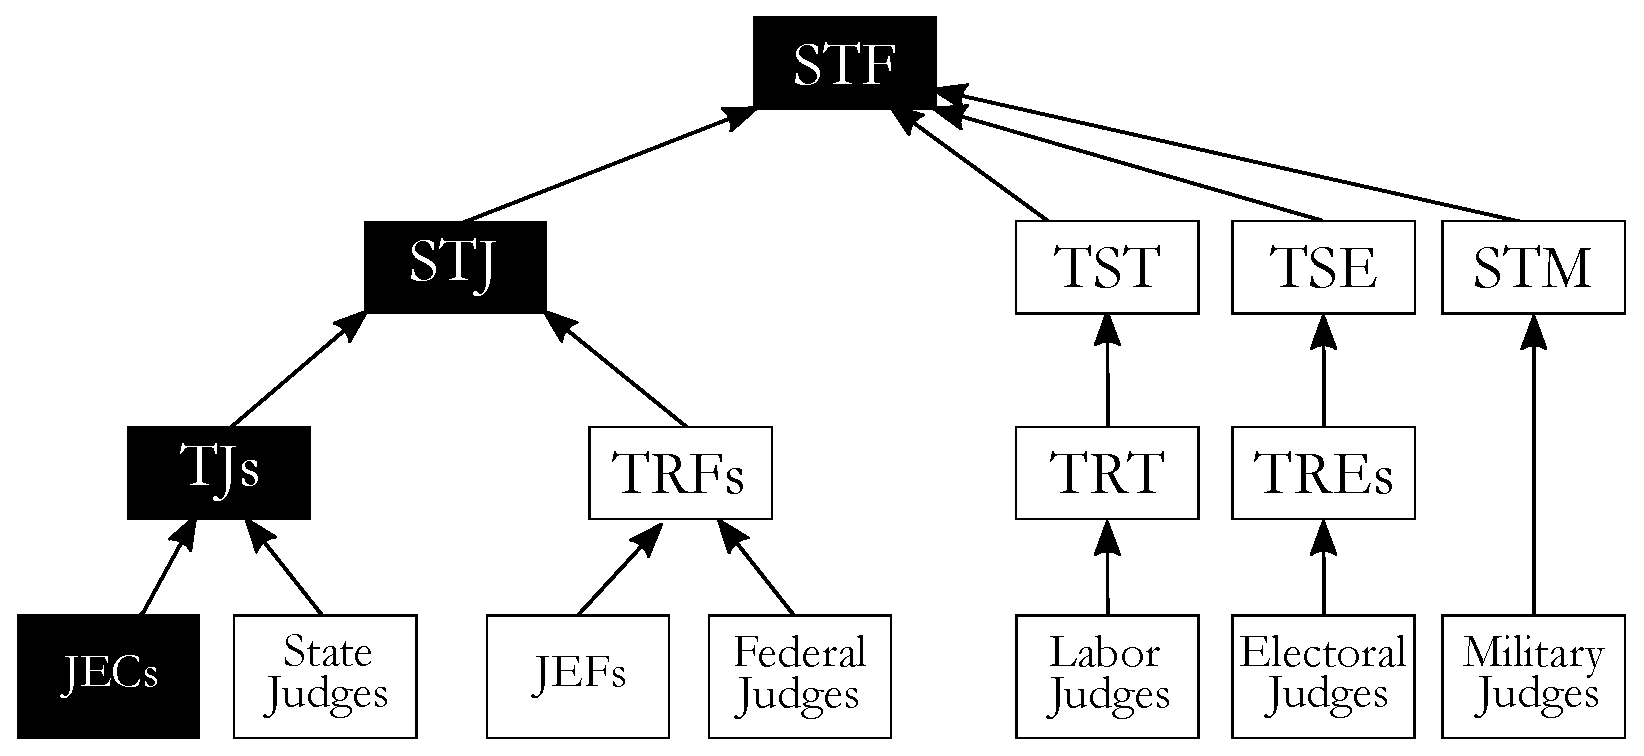
\includegraphics[width=0.8\textwidth]{images/chapters/fig1_courts.eps}
\end{figure}

Considering that the documents used in the task classification came from the \gls{JEC} at \gls{UFSC}, we follow the structure starting from \gls{JEC} at the lower level until the \gls{STF} at the top. As the higher courts judge the appeals of lower courts, the legal judgments' subjects from the higher courts may have a degree of similarity to the judgments from \gls{JEC}.

% Warning!! Copy/Paste 
Table~\ref{tab:count_process} shows the number of processes acquired and word count for each court.

\begin{table}[htb]
\caption{Acquired legal judgments from courts for embeddings training}
\label{tab:count_process}
\footnotesize
\centering
\begin{tabular}{@{}crrrr@{}}
\toprule
\textbf{Source}      & \multicolumn{1}{c}{\textbf{\begin{tabular}[c]{@{}c@{}}Collegial \\ Judgments\end{tabular}}}   & \multicolumn{1}{c}{\textbf{\begin{tabular}[c]{@{}c@{}}Individual \\ Judgments\end{tabular}}} & \multicolumn{1}{c}{\textbf{Subtotal}} &\multicolumn{1}{c}{\textbf{\begin{tabular}[c]{@{}c@{}}Word \\ Count\end{tabular}}} \\ \midrule
STF                  & 64,779              & 118,910              & 183,689     & 294,937,185  \\
STJ                  & 101,141              & 0                    & 101,141      & 312,687,450 \\
TJ-SC                & 989,964              & 662,535              & 1,652,499   & 3,060,212,814  \\
TJs (JusBrasil)           & 34,239               & 0                    & 34,239        & 78,138,337\\ \midrule
\multicolumn{1}{l}{} & \multicolumn{1}{l}{} & \textbf{TOTAL}       & 1,971,568     &  3,745,975,786\\ \bottomrule
\end{tabular}

%\fonte{\textcite{DalPont2020}.}
\end{table}

% Warning!! Copy/Paste 
After downloading all the legal judgments, most of them in \gls{PDF} and \gls{RTF}, we extracted raw texts from these files. We did not apply \gls{OCR} in scanned PDF documents, due to time limits to finish the experiments, so only digital \gls{PDF}  and \gls{RTF} files were accounted in Table~\ref{tab:count_process}. 

% Warning!! Copy/Paste 
With the extracted texts, we applied some preprocessing steps, as discussed further in this section. 

% Warning!! Copy/Paste 
Then we built the legal text corpora containing all the judgments related to all law subjects, which we call \emph{general} legal context corpora in this work. Using this base, we created another text corpora whose legal judgments are related only to air transport and consumer law, and we call it \emph{air transport} context corpora.

% Warning!! Copy/Paste 
To be able to compare how good embeddings trained with legal texts perform against those created with all kinds of texts, we also created other corpora from a variety of sources. Thus, we searched for free available textual datasets. In this work, we call these texts as \emph{global} context corpora. Table~\ref{tab:global_corpora} shows all the global text datasets used. Then we apply some preprocessing steps, as will be described further in this section.

\begin{table}[htb]
\caption{Global context corpora for embeddings training}
\label{tab:global_corpora}
\centering
\footnotesize
\begin{tabular}{@{}crrc@{}}
\toprule
\textbf{Dataset}                   & \textbf{Documents} & \textbf{Word Count} & \textbf{Source} \\ \midrule
Wikipedia in Portuguese            & 1,014,713          & 303,622,360         & \textcite{Wikipedia2019}                \\
Brazilian Literature Books         & 169                & 37,848,783          & \textcite{Tatman2017}                 \\
Old Newspapers                     & 617,627            & 26,441,581          &         \textcite{Tan2020}     \\
Folha de São Paulo News            & 165,641            & 74,594,367          &                     \textcite{Marlessonn2019}             \\
HC News Corpus                     & 494,128            & 27,170,063          &        \textcite{Christensen2016}         \\
Blogspot Posts                     & 2,181,073          & 696,657,915         &          \textcite{Santos2018}       \\
Wikihow Instructions               & 786,283            & 22,471,312          &        \textcite{Chocron2018}         \\ \midrule
\multicolumn{1}{r}{\textbf{TOTAL}} & 5,259,634          & 1,188,806,381       & \textbf{}       \\ \bottomrule
\end{tabular}

% \fonte{\textcite{DalPont2020}.}
\end{table}

The dataset for evaluation in the classification task is composed of almost one thousand legal judgments from the \gls{JEC} at \gls{UFSC}, issued between January 2014 to November 2019, and collected manually by a legal expert on site. The specific subject debated is failures in air transport services, such as flight delay, flight cancellation, baggage loss. Then the consumer injured claims compensation for immaterial damage, which is a monetary value fixed by the judge. 

% Não precisa
% The legal judgments refer only to situations in which consumers had problems with airlines. To solve them, the Code of Consumer Protection provides basic consumer's rights, such as effective compensation for material and immaterial damages, and ways to facilitate consumer's defense and ensure their rights. One of these is through Special Courts since it offers an unbureaucratic way out to solve their problems~\cite{Brazil1990}. 

% Não precisa
% Immaterial damage is an injury to personality rights, such as honor, dignity, intimacy, image, name~\cite{Goncalves2011}. Regarding the failures in air transport service, for example, flight delay, flight cancellation or baggage loss, the courts have been decided that they can generate immaterial damage and consumer compensation~\cite{Benjamim2015}. 

Compensation for immaterial damage is usually monetary. It is not possible to evaluate the painful sensation experienced by the injured person. As a mean of mitigating the consequences, money can play a satisfactory role~\cite{Diniz2020}. There are some circumstances considered by the judge when fixing the value, such as the person’s age, health status, person’s gender, place and time of injury. Anyway, these variables are weighted by the judge in a free assessment, according to his/her interpretation of each situation~\cite{Sadiku2020}.

A legal judgment is an unstructured textual document and refers to the final decision of a lawsuit in first degree. Generally, it consists of three elements~\cite{Brazil2015}:

\begin{itemize}[noitemsep]
    \item \emph{Report} (summary of what happened according to the parties allegations and evidences);
    \item \emph{Reasoning} (reasons that formed the judge's conviction);
    \item \emph{Result} (value fixed by the judge for immaterial damage compensation). 
\end{itemize}

There are four possible labels for the legal judgments:

\begin{itemize}[noitemsep]
    \item \textit{Well-founded:} The consumer wins the lawsuit, 26\% of the dataset.
    \item \textit{Not founded:} The consumer loses the lawsuit, 10\% of the dataset.
    \item \textit{Partly founded:} The consumer wins part of the lawsuit (for example, when he/she plead a greater compensation than the assigned value by the judge), 62\% of the dataset.
    \item \textit{Dismissed without prejudice:} The consumer makes a procedural error (for example, when he/she indicates as a defendant the wrong airline company). So the consumer can file a new lawsuit, 2\% of the dataset.
\end{itemize}

In the experiments from this section, to evaluate the representations using text classification, we removed the judgments' result part. Thus, to make predictions the \gls{ML} techniques will have the summary of the facts and the legal reasoning, that is the same data available at the early stages  of a real case.
Applying this approach, we could execute experiments while overcoming the difficulties of acquiring data from the early stages of lawsuits.

\subsection{Pipeline}\label{sec:pipeline_representation}

 
This section describes the pipelines and experimental setup for the experiments of embeddings training and evaluation.
 
The first part of the experiments consisted on training the word embeddings models based on  unlabeled corpora. 
%In such experiments, we used a set of programming tools such as Selenium \cite{Salunke2014}, to collect and extract the unlabeled corpora. Another set of tools was used to preprocess the text and train the embeddings, that is, \gls{NLTK} and  Gensim. At the end of this first part we had the trained word embeddings.
The second part of the experiments involved the evaluation of the embeddings in a text classification task of the legal judgments from \gls{JEC}, using the trained embeddings to represent the text.
 
Figure~\ref{fig:pipeline_embeddings} shows the pipeline used in the experiments from this section.
%pipeline for embeddings training and evaluation

\begin{figure}[htb]
    \centering
    \caption{Pipeline for embeddings training and evaluation}
    \label{fig:pipeline_embeddings}
    \includegraphics[width=\textwidth]{images/chapters/cap4_proposed_pipeline_embeddings.pdf}
\end{figure}

% Warning!! Copy/Paste

The pipeline from Figure~\ref{fig:pipeline_embeddings} receives three types of input: the unlabeled corpora, the legal judgments' text and the labels. In terms of output, there are three types: the trained embeddings, the classification models and the test set.

The first step in the pipeline is the text extraction, where the original files in \gls{PDF} and \gls{RTF} are converted to raw text format.
%
After text extraction, we applied some preprocessing steps, required before training the embeddings, as follows: the conversion to lower case and the removal of punctuation marks, special characters and symbol characters. We did not removed stopwords or apply stemmization or lemmatization, following the literature~\cite{Mikolov2013, Pennington2014}.


In the next step, there is the corpora split where the texts are divided in subsets. The three complete corpora comprised 3.7 billion, 100 million  and 1.19 billion words for \emph{general}, \emph{air transport} and \emph{global} corpora, respectively. The possible sizes of the subsets, considering word count are: 1,000; 10,000; 50,000; 100,000; 200,000; 500,000; 1,000,000; 5,000,000; 10,000,000; 25,000,000; 100,000,000; 500,000,000; 750,000,000 and 1,000,000,000.

We choose these corpora sizes to be able to compare the variation on performance metrics while increasing corpora size. For the air transport context, we could not embrace all these sizes due to limited corpora available. The largest subset for this context had 100 million words. 

Finally, each of the subsets (smaller corpora) was used to train distinct word embeddings representation.

As word embeddings technique, we had to choose one among the available one, such as Word2Vec, GloVe, and FastText, due to time limits to finish the experiments for publication. We chose GloVe  due to its good results in many \gls{NLP} tasks, including text classification, and also for its training time which is significantly lower than other techniques like Word2Vec and FastText~\cite{Pennington2014}.  
% Parâmetros do algoritmo
In terms of GloVe parameters, we kept most of the default values, except for windows size, training iterations (steps in one epoch), and output vector length, which were set to 5, 100, and 100, respectively. With these values, we achieved better results in text classification.

% Warning!! Copy/Paste
Considering the corpus sizes and the parameters described above, we trained fifteen representations for \emph{general} and fifteen for  \emph{global} context corpora. For \textit{air transport} context corpora, we trained eleven word embeddings.

% Warning!! Copy/Paste
To evaluate the GloVe embeddings representations, we applied each of them to the task of text classification of judgments from \gls{JEC} at \gls{UFSC}. 
As shown in Figure~\ref{fig:pipeline_embeddings}, the legal judgments' text and labels serve as input for the text classification pipeline. 

The next step is the text preprocessing, which is identical to the previous one, to reproduce the same textual structure used in the embeddings training. 
Using the Glove word embeddings, the text is numerically represented as detailed later.

To split the judgments in subsets for training and evaluation, we used the a random sampling method based on the proportions of 70\%, 15\% and 15\% for train, validation and test sets, respectively. The models use the train set during the train step, the validation set used to tune the models, and the test set at the end, as final evaluation.

Then, next step is the training of the classifiers. We used \gls{CNN} as a \gls{DL} classification technique based on the literature~\cite{Kim2014}. Figure~\ref{fig:cnn_model} illustrates this model.

\begin{figure}[htb]
    \centering
    \caption{CNN architecture for text classification}
    \label{fig:cnn_model}
    \includegraphics[width=\textwidth]{images/chapters/cnn_architecture.png}
    
    \fonte{\textcite{Kim2014}.}
\end{figure}

% Warning!! Copy/Paste
This \gls{CNN} takes into account the order of the words by stacking the corresponding embeddings for each word as they occur in the text. 
% Warning!! Copy/Paste
Then it applies multiple convolutional masks with different dimensions that correspond to the red and yellow contours in Figure~\ref{fig:cnn_model}. Mask widths are equal to word embedding size while the heights can vary. In this context, mask height can be related to the idea of N-Grams, since they embrace multiple embeddings at the same time. 
% Warning!! Copy/Paste
In the original architecture, these heights were set to three, four, and five. We added one more mask of height two, which increased classification metrics. Also, based on empirical experimentation, we set  the number of masks to ten for each of these sizes, without affecting our results, but decreasing the required training time. 

% Warning!! Copy/Paste
% Explicar sobre como esse modelo foi utilizado
In this work, we applied each of the embeddings trained in conjunction with the \gls{CNN} described to the classification of \gls{JEC} at \gls{UFSC} judgments, where Out of Vocabulary (OOV) words are replaced by an vector of random values. Thus, we trained and tested 41 models. Furthermore, due to the stochastic nature of neural networks training methods~\cite{Cohen1995}, each of these models was trained and tested 200 times and the resulting evaluation metrics were averaged. 

% Warning!! Copy/Paste
Finally, we compare the performance in classification using accuracy and macro F1-Score.


\subsection{Results and Discussion}

% Warning!! Copy/Paste
Following the steps presented in Section~\ref{sec:pipeline_representation}, we trained all 41 word embeddings representations for GloVe. 

% Warning!! Copy/Paste
To illustrate how these embeddings behave, Figure~\ref{fig:projection} shows the projection in two dimensions, using \gls{t-SNE} \cite{Maaten2008} of perplexity of 0.1, of a sample of words from \emph{general} context embedding trained with 1 billion words. Each axis corresponds to a \gls{PC}.

\begin{figure}[tb]
    \centering
    \caption{Word Embeddings projection using t-SNE}
    \label{fig:projection}
    \includegraphics[width=\textwidth]{images/chapters/tsne_2000_0.1.pdf}
    
    % \fonte{\textcite{DalPont2020}.}
\end{figure}

% Warning!! Copy/Paste
%%%% FIGURE- Embeddings projection
%Using each embedding, we trained and tested  \gls{CNN} for text classification of the judgments from \gls{JEC}. %These two steps were repeated 200 times, and the evaluation metrics were averaged for each group of repetitions.

% Warning!! Copy/Paste
In Figure~\ref{fig:accuracy_plot} and \ref{fig:f1_plot}, we present the results, for accuracy and F1-Score, respectively, from test data applied to each \gls{CNN}. These results are related to pre-trained embeddings  with \emph{general}, \emph{air transport}, \emph{global} texts. 
The x-axis denotes the corpus sizes used to train the embeddings, while the y-axis represents accuracy or F1-Score. Each data point represents the average of the evaluation metric, after 200 train and test repetitions using each specific embedding. %Finally, we delimited y-axis to smaller intervals so the metrics variations could be visible.


% JH In the next section, we discuss these results.

\begin{figure}[htb]
    \centering
    \caption{Accuracy for test set from CNN in embeddings evaluation}
    \label{fig:accuracy_plot}
    \includegraphics[width=\textwidth]{images/chapters/acc_mean_final.pdf}
    
    % \fonte{\textcite{DalPont2020}.}
\end{figure}

\begin{figure}[htb]
    \centering
    \caption{Macro F1-Score for test set from CNN  in embeddings evaluation}
    \label{fig:f1_plot}
    \includegraphics[width=\textwidth]{images/chapters/f1_score_mean_final.pdf}
    
    % \fonte{\textcite{DalPont2020}.}
\end{figure}

% Evaluations from context perspective
%\subsection{Discussion from Context Perspective}

% Warning!! Copy/Paste
We focus now on the part of research question regarding specificity: Does the \textit{specificity}  of the corpus used for word embeddings training impact the performance of a text classification using such representations? 

% Warning!! Copy/Paste
In terms of accuracy, when we compare \emph{global} against others (Figure~\ref{fig:accuracy_plot}), we have that higher text specificity leads to better results, for most of the corpus sizes used for embeddings training. Furthermore, when comparing \emph{general} and \emph{air transport} curves, there is a significant difference in accuracy only for the lowest and highest x-values. 
However, in terms of F1-Score, as shown in Figure~\ref{fig:f1_plot}, our observations change, once \emph{general} and \emph{air transport} curves have a similar shape. Also, for the highest corpus sizes, \emph{general} and \emph{global} curves converge to similar values of F1-Score. 
%
% Warning!! Copy/Paste
The differences in accuracy and F1-Score may emerge from the fact that our dataset to text classification is imbalanced, once the former does not take this fact into account, while the latter does. However, this result still requires further investigation. 
% Warning!! Copy/Paste
% In general, we can note that for smaller corpora sizes for embeddings training, text specificity has a more impact than for large sizes.


%\subsection{Discussion from Corpus Size Perspective}

% Warning!! Copy/Paste
Regarding the part of research question in terms of size: 
Does the \textit{size}  of the corpus used for word embeddings training impact the performance of a text classification using such representations? 

% Warning!! Copy/Paste
When we observe both accuracy and F1-Score measures from Figure~\ref{fig:accuracy_plot} and \ref{fig:f1_plot}, it is clear the tendency for improvement while increasing corpus size. However, the metrics converge with the largest corpus sizes. There are two exceptions. The first one occurs with smaller values of corpus sizes for \textit{global} curve, as it decreases in F1-Score measures. The second corresponds to the last data point in \textit{air transport} curves. The former can happen when the classifier performs poorly for some classes while gets better in others. The latter may indicate that those curves could improve if we had more significant corpus sizes related to that context.

% Warning!! Copy/Paste
In general, we can note that the greater the corpus size in embeddings training, the better are the results. However, this impact decreases as the corpus size increases until a point where more words in the corpus have little impact on the results.

\section{Text Classification in Legal Judgments}\label{sec:text_classification}

% Explain the overall idea of the experiments

% How did we get to this setup?

% É possível usar TM techniques para classificar corretamente as sentenças?

This section presents the results for the classification experiments involving \gls{JEC}'s legal judgments. The section starts from the clarification of the experiments' purpose, that is, how they help on answering the research question. Then, it presents the details on the datasets used for the experiments, the pipelines of the experiments for Classical \gls{ML} and \gls{DL}, and the results and discussion.

\subsection{Experiment's Purpose}

% \begin{itemize}[noitemsep]
%     \item Primeiro experimento
%     \item Sentir dificuldades
%     \item Tornar compreensível a pipeline para o especialista
%     \item orange 3 - técnicas classicas
%     \item Como ele ajuda a responder  à segunda parte pergunta?
% \end{itemize}


The experiments' purpose is to answer the second part of the research question, that is, whether \gls{DL} techniques  can achieve better performance on \gls{JEC}'s cases classification when compared to Classical \gls{ML} techniques.
% Detail here.
Through the application of Classical and \gls{DL} techniques to the prediction of the \gls{JEC} legal judgments, we try to estimate the techniques' performance. 
Based on the results, we compare the techniques on how well they perform.

Besides the techniques comparison, in this section we tested the performance of the models using two datasets: legal judgments with full text and the legal judgments without the results section. Using  such strategy, one can notice whether including or not the results part, containing textual description of the label, impact in the models performance. 


In the experiments with Classical \gls{ML} techniques, we applied the open-source software Orange Data Mining (Version 3.22)~\cite{Demsar13}. Such tool aims at offering a variety of \gls{ML} and \gls{TM} techniques to the user in a simple way, without the need of any programming language. On the other hand, the experiments with \gls{DL} techniques (not available in Orange) required the use of several tools: the Python programming language, version 3.8; the Keras framework,Version 2.4.3~\cite{Chollet2015}; the Natural Language Toolkit (NLTK), version 3.5 ~\cite{Loper02} and the Scikit-Learn framework, version 0.24.1~\cite{Pedregosa2012}.\footnote{Pipeline for Orange3 and code for Keras are available at \url{https://github.com/thiagordp/text_classification_in_legal_docs}.}


Finally, the results presented in this section relate to the first contact of the researcher with the areas of study. Thus, considering the extensive amount of publications on legal text classification (detailed in Appendix~\ref{ap:rsl_ml_law}) and the researcher's expertise, the classification experiments produced small contributions, that is, the applications of Classical \gls{ML} and \gls{DL} techniques to the prediction of the results of legal judgments from \gls{JEC}.


\subsection{Datasets}

For the classification experiments, two datasets were used. Both are similar as before (JEC/UFSC legal judgments), but smaller because it was the first experiment performed. The judgments were issued between  January 2014 to May 2019.

The difference in the legal judgments from the two datasets used resides in their distinct textual structure.  In one of them, we removed the result's part, while in the other dataset,  we kept such part. Thus, considering the structure of a legal judgment described in Section~\ref{sec:embedding_dataset}, the first dataset contains legal judgments composed of two parts and less amount of text. The second dataset has three parts and more text.

Table~\ref{tab:cap4_class_distr_label} describes the quantity of examples for each label. 

\begin{table}[htb]
\centering
\caption{Label's distributions for text classification}
\label{tab:cap4_class_distr_label}
\footnotesize
\begin{tabular}{@{}lc@{}}
\toprule
\multicolumn{1}{c}{\textbf{Label}} & \textbf{Examples} \\ \midrule
Well Founded                            & 214               \\
Partly Founded                     & 379               \\
Dismissed without prejudice        & 10                \\
Not founded                        & 70                \\ \midrule
\multicolumn{1}{r}{\textbf{TOTAL}} & 673               \\ \bottomrule
\end{tabular}
\end{table}


In terms of quantitative information from the datasets, Table~\ref{tab:info_dataset_classification} presents the average count of tokens per document and the vocabulary size after each of the preprocessing steps for each dataset. As we will describe later, distinct preprocessing steps carried out for the experiments with Classical \gls{ML} and \gls{DL}. The information of tokens per document in the experiment with Classical ML was not available due to the restrictions from Orange Data Mining.


\begin{table}[htb]
\centering
\caption{Information on the datasets for classification}
\label{tab:info_dataset_classification}
\footnotesize
\begin{tabular}{@{}crrrr@{}}
\toprule
\textbf{\begin{tabular}[c]{@{}c@{}}Experiment's\\ Preprocessing\end{tabular}} & \multicolumn{1}{c}{\textbf{\begin{tabular}[c]{@{}c@{}}Tokens per \\ document\\ (w/ result)\end{tabular}}} & \multicolumn{1}{c}{\textbf{\begin{tabular}[c]{@{}c@{}}Vocabulary Size\\ (w/ result)\end{tabular}}} & \multicolumn{1}{c}{\textbf{\begin{tabular}[c]{@{}c@{}}Tokens per \\ document\\ (w/o result)\end{tabular}}} & \multicolumn{1}{c}{\textbf{\begin{tabular}[c]{@{}c@{}}Vocabulary Size\\ (w/o result)\end{tabular}}} \\ \midrule
\textbf{Classical ML}                                                         & -                                                                                                         & 12,994                                                                                                 & -                                                                                                          & 12,898                                                                                                   \\
\textbf{DL}                                                                   & 673.0                                                                                                         & 15,377                                                                                                  & 644.2                                                                                                          & 15,224                                                                                                   \\ \bottomrule
\end{tabular}
\end{table}

Similar to Section~\ref{sec:text_representation}, some of the legal judgments from the datasets presented more than one result, that is, they had more than one distinct labels. An example of this type of judgments happens when two people file a joint lawsuit against an airline, and the judge set distinct judgments for each of them. In those cases, the documents were replicated for each of the labels indicated on its results section, culminating in a total of 673 legal judgments, in each dataset, to serve as input for the experiments. Considering distinct legal judgments only, the dataset contains 665 documents.



% Cases' result = label in this work

\subsection{Pipelines}

This section describes the pipelines and experimental setup for the experiments with Classical \gls{ML} and \gls{DL} techniques.

The first set of classification experiments focused on the application of Classical \gls{ML} techniques. In such experiments, Orange 3 served as execution environment and followed the pipeline from Figure~\ref{fig:cap4_pipeline_superv_ml}. It receives two types of input: the texts from legal judgments, in a plain text format, and their labels, that is, the judgments' results. As outputs, the pipeline makes available the trained models and the test set which are passed to the prediction and evaluation step.


\begin{figure}[htb]
    \centering
    \caption{Pipeline for legal text classification using Classical ML techniques}
    \label{fig:cap4_pipeline_superv_ml}
    \includegraphics[width=\textwidth]{images/chapters/cap4_classification_pipeline.pdf}
\end{figure}


The first step in the pipeline is the data preprocessing. Considering the available techniques for preprocessing textual data, described in Chapter 2 and in the literature, in Appendix~\ref{ap:rsl_ml_law},  we applied transformation, tokenization, stemming and filtering, previously discussed in Section \ref{sec:bow}:

\begin{itemize}[noitemsep]
    \item \textbf{Tranformation:} the conversion to lower case to standardize the spelling of words.
    \item \textbf{Tokenization:} the application of regular expression ($\setminus w+$) to detect the pieces of texts, while removing spaces, symbols, and punctuation.
    \item \textbf{Stemming:} To reduce the variability of similar words, we applied Porter Stemmer~\cite{Porter1980}, a simple and efficient stemming algorithm to the Portuguese language. However, it may make errors, such as contracting the word \textit{morais} to \textit{morai}, instead of \textit{moral} (Portuguese words for singular and plural of \textit{moral}, respectively).
    \item \textbf{Filtering:} Removing stopwords, such as prepositions and articles to keep only the meaningful words.
\end{itemize}


The next step in the pipeline relates to the extraction of N-Grams, which detects sequences of two or more words that appear together consistently in the text. In this research, the limit of the length of N-grams was two. Bigger numbers of N-grams would lead to large textual representations.



After N-Grams Extraction, the numerical representations of the documents are created using the algorithm \gls{BOW}. In the experiments with Classical \gls{ML}, we used the \gls{TF} to calculate the values of the BOW model. 


The next step consists on dividing the dataset in two subsets: train and test sets. As described in Chapter~\ref{cap:ml_text}, there is the cross validation. In this research, $k$ was set to 10, that is, 90\% of the dataset used for training and 10\% for testing the models. Such proportion is a common choice to avoid bias while keeping some level of variance in the division of the folds~\cite{Airola2011}

The next step consists on training the models to predict the result of the judgments from \gls{JEC} according to the possible outcomes, as described in Section~\ref{sec:text_representation}. 
Experiments involved the following techniques: \gls{kNN}, \gls{SVM}, \gls{RF}, \gls{NN}, \gls{NB} and \gls{LR}. Table~\ref{tab:hyperparam_classification} presents the hyper-parameters applied to each technique, based on the values suggested by Orange 3.


% Incluir Tabela para descrever os parâmetros dos modelos.
\begin{table}[htb]
\centering
\caption{Hyperparameters for classification techniques}
\label{tab:hyperparam_classification}
\footnotesize
\begin{tabular}{cl}
\toprule
\textbf{Technique} & \multicolumn{1}{c}{\textbf{Hyper-parameters}} \\ \midrule

\gls{kNN} & \begin{tabular}[c]{@{}l@{}}Number of Neighbors: 4;\\ Distance Metric: Euclidean;\\ Weight: Uniform\end{tabular} \\ \hdashline

\gls{LR} & \begin{tabular}[c]{@{}l@{}}Regularization type: Ridge (L2);\\ C (strength): 1\end{tabular} \\\hdashline

\gls{NB} & -- \\ \hdashline

\gls{NN} & \begin{tabular}[c]{@{}l@{}}Hidden Layers: 2\\ Neurons in each layer: 100, 50;\\ Activation Function: tanh;\\ Solver: Stochastic Gradient descent (SGD)\end{tabular} \\ \hdashline

\gls{RF} & \begin{tabular}[c]{@{}l@{}}Number of Trees: 10;\\ Minimum subset size: 5\end{tabular} \\ \hdashline

\gls{SVM} & \begin{tabular}[c]{@{}l@{}}C (cost): 1.0;\\ $\epsilon$ (Regression loss): 0.1;\\ Kernel: \gls{RBF};\\ Iteration Limit: 100\end{tabular} \\ \bottomrule

\end{tabular}
\end{table}


Finally, there is the evaluation step, which estimates how well the models performed on predicting unseen legal judgments. To measure the performance, we used the Accuracy, detailed in Chapter~\ref{cap:ml_text}. At the time these experiments were published, only the accuracy was used.

The second set of experiments related to the application of \gls{DL} techniques to the prediction of the legal judgments' results. The pipeline used for these experiments is presented in Figure~\ref{fig:pipeline_dl}.

\begin{figure}[htb]
    \centering
    \caption{Pipeline for legal text classification using DL techniques}
    \label{fig:pipeline_dl}
    \includegraphics[width=\textwidth]{images/chapters/cap4_proposed_pipeline_dl.pdf}
\end{figure}

Such steps in the pipeline are similar to those in Figure~\ref{fig:cap4_pipeline_superv_ml}, however there are distinct settings. 
Thus, the pipeline receives three types of input: the legal judgments' text, their labels and the pre-trained word embeddings  models. 

Following, the preprocessing step prepares the text to the next steps in the pipeline, however with  different settings from Figure~\ref{fig:cap4_pipeline_superv_ml}. There is the transformation, tokenization using regular expression (\textbackslash w+), however we did not apply stemming or filtering, following the literature~\cite{Mikolov2013, Pennington2014}. Thus, to reproduce the aspects of the corpus applied to the pre-training of the embeddings, their application in ML tasks may not include those preprocessing techniques.
After preprocessing there is the text representation, where pre-trained embeddings techniques were applied. We selected the pre-trained embeddings based on best results in Section~\ref{sec:text_representation}. That is, the word embeddings pre-trained using the corpus related to air transport only. In the referred section, only the GloVe technique was applied and tested due to time limits. However, we later trained other word embeddings in the same corpora to apply in the classification experiments, using the default parameters from Gensim~\cite{Radim2010}.

The next step, cross-validation,  follows the setup from the Classical ML experiments, i.e., the number of folds set to ten. 

Later, there is the models training step, involving three \gls{DL} techniques: \gls{CNN}, \gls{LSTM} and Bi-LSTM with Self Attention. The \gls{CNN} used has the same hyperparemeters  from Section~\ref{sec:text_representation}. 

The \gls{LSTM} architecture, as shown in Figure~\ref{fig:cap4_lstm_model}, receives as input the embeddings, which can be fine-tuned during the training process. Such a setting is enabled in this architecture. The embeddings pass to a Spatial Dropout layer, a regularization method to avoid overfitting on recurrent networks, especially when embeddings can be fine-tuned~\cite{Gal2016}. Then, there is the \gls{LSTM} layer with $100$ units with a dropout and a recurrent dropout of $0.2$. Finally, the output layer corresponds to a Dense Layer with four neurons having sigmoid as activation function.

\begin{figure}[htb]
    \centering
    \caption{LSTM architecture for text classification}
    \label{fig:cap4_lstm_model}
    \includegraphics[width=\textwidth]{images/chapters/cap4_lstm_model.pdf}
\end{figure}

% TODO: Definir no C2, LSTM, CNN, Bi-LSTM e Self Attention
The architecture for Bi-LSTM with Self Attention is shown in Figure~\ref{fig:cap4_bilstm_attention_model}. It starts with the Embedding layer followed by Spatial Dropout, both with the same settings from previous \gls{LSTM} model. The Bi-LSTM layer follows, containing 100 units. Then, there is the Many to One Attention step composed of  the Self-Attention, the Concatenation with last Bi-LSTM Hidden State and the Attention Vector. Finally, there is the Dense Layer as the output layer with four neurons with sigmoid activation function.

\begin{figure}[htb]
    \centering
    \caption{Bi-LSTM with Self-Attention architecture for text classification}
    \label{fig:cap4_bilstm_attention_model}
    \includegraphics[width=\textwidth]{images/chapters/cap4_bi-lstm_self_attention_model.pdf}
\end{figure}

% Adam with default parameters from Keras.

To run the \gls{DL} experiments based on the architecture from Figure~\ref{fig:pipeline_dl}, distinct setups have been made considering the three \gls{DL} techniques, the two datasets, and the five embeddings models. %Thus, there were thirty combinations of inputs in the experiments.


\subsection{Results and Discussion}


The results obtained after applying the sets of input to the pipelines from Figure~\ref{fig:cap4_pipeline_superv_ml} and~\ref{fig:pipeline_dl} are presented in the following paragraphs.
%
Table~\ref{tab:cap4_class_with_result} details the accuracy obtained by the techniques and representations on each label using the full judgments' text.

% Please add the following required packages to your document preamble:
% \usepackage{booktabs}
% \caption{Acurácia da classificação com o dispositivo das sentenças}
\begin{table}[htb]
\centering
\caption{Classification accuracy for the dataset with judgments' result}
\label{tab:cap4_class_with_result}
\footnotesize
\begin{tabular}{@{}cccrrrrr@{}}
\toprule
\textbf{Technique}&\multicolumn{1}{c}{\textbf{\begin{tabular}[c]{@{}c@{}}Type of\\\gls{ML}\\technique\end{tabular}}} & \textbf{Representation} & \multicolumn{1}{c}{\textbf{\begin{tabular}[c]{@{}c@{}}Well\\ founded\end{tabular}}} & \multicolumn{1}{c}{\textbf{\begin{tabular}[c]{@{}c@{}}Partly\\ founded\end{tabular}}} & \multicolumn{1}{c}{\textbf{\begin{tabular}[c]{@{}c@{}}Not\\ founded\end{tabular}}} & \multicolumn{1}{c}{\textbf{\begin{tabular}[c]{@{}c@{}}Dismissed\\ without\\ prejudice\end{tabular}}} & \multicolumn{1}{c}{\textbf{\begin{tabular}[c]{@{}c@{}}Total\\Acc\end{tabular}}} \\ \midrule
\textbf{\gls{kNN}} & Classical & BOW TF & 75,9\% & 71,9\% & 93,5\% & 95,7\% & 75,8\% \\
\textbf{\gls{LR}} & Classical  & BOW TF & 87,1\% & 86,2\% & 97,6\% & 97,9\% & 87,8\% \\
\textbf{\gls{NB}} & Classical  & BOW TF & 75,2\% & 47,3\% & 91,4\% & 19,6\% & 60,3\% \\
\textbf{\gls{NN}} & Classical  & BOW TF & 85,9\% & 84,9\% & 97,5\% & 97,9\% & 86,7\% \\
\textbf{\gls{RF}} & Classical  & BOW TF & 82,6\% & 82,6\% & 96,1\% & 97,9\% & 84,2\% \\
\textbf{\gls{SVM}} & Classical  & BOW TF & 34,3\% & 45,5\% & 89,6\% & 98,5\% & 47,3\% \\
\textbf{Bi-LSTM-SA} & \gls{DL}& FT CBOW & 81,1\% & 80,4\% & 96,6\% & 98,2\% & 78,1\% \\
\textbf{Bi-LSTM-SA} & \gls{DL} & FT \gls{SG} & 81,1\% & 80,2\% & 97,3\% & 98,5\% & 78,6\% \\
\textbf{Bi-LSTM-SA}  & \gls{DL} & GloVe & 83,1\% & 82,6\% & 96,9\% & 98,2\% & 80,4\% \\
\textbf{Bi-LSTM-SA} & \gls{DL}  & W2V CBOW & 81,3\% & 80,1\% & 97,5\% & 98,4\% & 78,6\% \\
\textbf{Bi-LSTM-SA}  & \gls{DL} & W2V \gls{SG} & 80,8\% & 79,6\% & 97,5\% & 98,4\% & 78,2\% \\
\textbf{\gls{CNN}} & \gls{DL}  & FT CBOW & 48,3\% & 48,9\% & 90,2\% & 98,5\% & 42,9\% \\
\textbf{\gls{CNN}} & \gls{DL}  & FT \gls{SG} & 94,0\% & 94,8\% & 96,9\% & 98,5\% & 92,1\% \\
\textbf{\gls{CNN}}  & \gls{DL} & GloVe & \textbf{97,2\%} & \textbf{97,5\%} & \textbf{98,1\%} & 98,4\% & \textbf{95,5\%} \\
\textbf{\gls{CNN}}  & \gls{DL} & W2V CBOW & 73,0\% & 68,7\% & 90,6\% & 98,5\% & 65,4\% \\
\textbf{\gls{CNN}} & \gls{DL}  & W2V \gls{SG} & 96,0\% & 96,9\% & 97,6\% & 98,5\% & 94,5\% \\
\textbf{\gls{LSTM}} & \gls{DL}  & FT CBOW & 78,2\% & 74,6\% & 90,5\% & 98,5\% & 70,9\% \\
\textbf{\gls{LSTM}}  & \gls{DL} & FT \gls{SG} & 80,2\% & 76,4\% & 92,9\% & 98,5\% & 74,0\% \\
\textbf{\gls{LSTM}} & \gls{DL}  & GloVe & 80,7\% & 78,6\% & 96,1\% & 98,5\% & 77,0\% \\
\textbf{\gls{LSTM}}  & \gls{DL} & W2V CBOW & 77,4\% & 73,8\% & 89,6\% & 98,5\% & 69,7\% \\
\textbf{\gls{LSTM}} & \gls{DL}  & W2V \gls{SG} & 78,6\% & 73,7\% & 91,8\% & 98,5\% & 71,3\% \\ \bottomrule
\end{tabular}

%\fonte{\textcite{Sabo2019}.}
\end{table}


% O que escrever aqui?
% Primeiro dizer o óbvio: qual a ordem da melhor pra pior?
% CNNs..., LR e tudo mais
% CNN foi muito bem, soube detectar bem quais palavras tem alguma relação com o resultado.
% E as demais técnicas, o que mudou?
% Diferença entre os resultados dos embeddings.
% Em relação às classes? continua igual?
% WF: CNN Glove, W2V SG, FT SG, 
% PF: idme
% NF:
% DWJ: 
% TOAL:
% Pq? 
% - Possíveis causas para bom resultado:
%       Facilidade em relacionar o texto descrito com o resultado, mas não uma capacidade de "raciocinar" 


From Table~\ref{tab:cap4_class_with_result}, one can notice that most techniques achieved accuracies superior to 70\%, indicating good results on the classification of legal judgments from \gls{JEC}. In terms of techniques' performances, the CNN with GloVe embeddings achieved the best accuracies for the  \emph{Well Founded}, \emph{Partially Founded},  \emph{Not founded} labels and for the total accuracy. The \gls{CNN} also achieve good results when combined with the Word2Vec \gls{SG} and FastText \gls{SG}. Besides \gls{CNN}, the next techniques with best performances are Classical \gls{ML} techniques, that is, \gls{LR}, \gls{NN} and \gls{RF}. 

In terms of worst results, the \gls{CNN} with FastText \gls{CBOW} embeddings achieved the smallest total accuracy, followed by \gls{SVM}, Naïve Bayes and \gls{CNN} with Word2Vec CBOW. Regarding labels, on the other hand,  \gls{SVM} achieved the worst results for the  \emph{Well Founded}, \emph{Partially Founded},  \emph{Not founded}, and the Naïve Bayes for the \emph{Dismissed without Prejudice} label.



The second part of experiments on Classical \gls{ML} and \gls{DL} related to the classification of legal judgments from \gls{JEC} without the judgments' result. Table~\ref{tab:cap4_class_without_result} contains the accuracy achieved by each technique and representation for the four labels and total accuracy using the text of the judgments without result. 


\begin{table}[htb]
\centering
\caption{Classification accuracy for the dataset without judgments' result}
\label{tab:cap4_class_without_result}
\footnotesize
\begin{tabular}{@{}cccrrrrr@{}}
\toprule
\textbf{Technique} &\multicolumn{1}{c}{\textbf{\begin{tabular}[c]{@{}c@{}}Type of\\\gls{ML}\\technique\end{tabular}}} & \textbf{Representation} & \multicolumn{1}{c}{\textbf{\begin{tabular}[c]{@{}c@{}}Well\\ Founded\end{tabular}}} & \multicolumn{1}{c}{\textbf{\begin{tabular}[c]{@{}c@{}}Partly\\ founded\end{tabular}}} & \multicolumn{1}{c}{\textbf{\begin{tabular}[c]{@{}c@{}}Not\\ founded\end{tabular}}} & \multicolumn{1}{c}{\textbf{\begin{tabular}[c]{@{}c@{}}Dismissed\\ without\\ prejudice\end{tabular}}} & \multicolumn{1}{c}{\textbf{\begin{tabular}[c]{@{}c@{}}Total\\Acc\end{tabular}}} \\ \midrule
\textbf{kNN} & Classical & BOW TF & 75,2\% & 72,1\% & 90,9\% & 93,2\% & 75,4\% \\
\textbf{LR} & Classical  & BOW TF & 80,7\% & 79,2\% & 94,9\% & 97,9\% & 81,6\% \\
\textbf{NB} & Classical  & BOW TF & 74,3\% & 46,5\% & 90,2\% & 18,1\% & 59,5\% \\
\textbf{NN} & Classical  & BOW TF & 81,0\% & 79,0\% &\textbf{ 95,1\%} & 97,9\% & 81,6\% \\
\textbf{RF}  & Classical & BOW TF & \textbf{82,2\%} & \textbf{79,9\%} & 92,7\% & 97,9\% & \textbf{82,2\%} \\
\textbf{\gls{SVM}} & Classical  & BOW TF & 33,4\% & 45,0\% & 89,6\% & 98,5\% & 46,7\% \\
\textbf{Bi-LSTM-SA} & \gls{DL} & FT CBOW & 79,5\% & 77,1\% & 94,3\% & 98,5\% & 74,7\% \\
\textbf{Bi-LSTM-SA}  & \gls{DL} & FT \gls{SG} & 78,5\% & 75,8\% & 94,6\% & 98,5\% & 73,7\% \\
\textbf{Bi-LSTM-SA}  & \gls{DL} & GloVe & 79,9\% & 77,3\% & 94,8\% & 98,4\% & 75,2\% \\
\textbf{Bi-LSTM-SA} & \gls{DL}  & W2V CBOW & 79,5\% & 76,7\% & 93,9\% & 98,5\% & 74,3\% \\
\textbf{Bi-LSTM-SA}  & \gls{DL} & W2V \gls{SG} & 80,4\% & 77,4\% & 93,8\% & 98,5\% & 75,0\% \\
\textbf{CNN}  & \gls{DL} & FT CBOW & 50,5\% & 51,7\% & 89,9\% & 98,5\% & 45,3\% \\
\textbf{CNN}  & \gls{DL} & FT \gls{SG} & 80,8\% & 78,0\% & 93,0\% & 98,5\% & 75,2\% \\
\textbf{CNN} & \gls{DL}  & GloVe & 80,4\% & 77,3\% & 93,0\% & 98,5\% & 74,6\% \\
\textbf{CNN}  & \gls{DL} & W2V CBOW & 66,6\% & 58,7\% & 90,0\% & 98,5\% & 56,9\% \\
\textbf{CNN} & \gls{DL}  & W2V \gls{SG} & 81,7\% & 79,5\% & 93,3\% & 98,5\% & 76,5\% \\
\textbf{LSTM}  & \gls{DL} & FT CBOW & 79,8\% & 71,3\% & 88,6\% & 98,5\% & 69,1\% \\
\textbf{LSTM}  & \gls{DL} & FT \gls{SG} & 77,5\% & 69,1\% & 88,1\% & 98,5\% & 66,6\% \\
\textbf{LSTM} & \gls{DL}  & GloVe & 81,1\% & 74,7\% & 91,2\% & 98,5\% & 72,8\% \\
\textbf{LSTM}  & \gls{DL} & W2V CBOW & 80,8\% & 73,7\% & 87,8\% & 98,5\% & 70,4\% \\
\textbf{LSTM} & \gls{DL}  & W2V \gls{SG} & 79,2\% & 72,4\% & 88,4\% & 98,5\% & 69,2\% \\ \bottomrule
\end{tabular}

%\fonte{\textcite{Sabo2019}.}
\end{table}

The results show the sequence of best techniques has changed, as the Classical ML techniques \gls{RF}, \gls{LR} and \gls{NN} achieved the best total accuracies followed by the \gls{CNN} with Word2Vec \gls{SG}. In terms of labels, the RF performed better for the \emph{Well founded} and  \emph{Partially founded}, while \gls{NN} performed better with \emph{Not founded}. For the label \textit{Dismissed without prejudice}, several classes achieved good results, although it has the smallest sample. On the other hand, similar to the results from Table~\ref{tab:cap4_class_with_result}, the techniques with worse performance were the \gls{CNN} with FastText CBOW followed by \gls{SVM} and \gls{CNN} with Word2Vec CBOW.


% Results para colocar aqui
% 
% A CNN ele se saiu muito bem com resultado e não tão bem sem  o resultado o que mostra que ela conseguiu relacionar muito bem o trecho da sentença com o label do doc, isto é. A CNN identificou a sentença como uma parte muito importante do documento.
% Além disso, percebeu-se a importância da técnicna de representação, uma que vez que simplesmente alterando a representação utilizada na CNN fez que com ela tivesse tanto resultados muito bons quanto muito ruins.
% Deixar claro que o caso prático seria usar o texto sem a sentença final, apenas contentdo o resumo do caso e as leis aplicáveis. Portanto que num caso real no JEC, as técnicas de Classical ML seriam mais adequadas para a classificação.


In general, it is inferred that the accuracy in the experiment with the removal of the judgments' result (part of the text indicating the label to which it belongs) suffered a minimal reduction for the Classical ML techniques as well as LSTM and Bi-LSTM-SA, which demonstrates that the classifiers were able to maintain their performance with the text in which the facts narrated by the parties to the process are reported and the legal grounds applicable to the case. 
However, for the CNN there was a significant decay in performance when removing the cases' result. And, such  decay in performance may show the technique inferred that the text from the result part  had significant information for the classification of the legal cases.
However, the removal of such part made it harder for the CNN to infer the judgment's label based on remaining two parts of the text. 

Another observation for the CNN is the impact of the representations in the performance of the technique, as changing the representation used in the pipeline was enough to reduce the accuracy by more than 30\% when comparing to the best CNN results. However, for the other two DL techniques, LSTM and Bi-LSTM with Self Attention, the differences in performance while shifting representations were significantly smaller.

% Esse fica como último parágrafo.
Finally, a good performance when classifying the judgments without results becomes a prerequisite for carrying out experiments with texts from legal proceedings in which there is still no sentence, that is, in which the judge has not yet decided the result. In this case, the best choice may be the use of Classical ML techniques, such as LR and RF, as they perform better on the classification task than DL techniques and due to the fact those models are less complex and require less examples to train.
The \gls{DL} techniques, especially CNN with GloVe may be useful inside JEC when the objective is to organize existing judgments by categories such as their labels or matters, for example. 

This conclusions are limited to our small dataset from \gls{JEC}. Thus, if we had a larger dataset with more training examples, the \gls{DL} would possibly achieve better results.


% Place this in Conclusions Chapter
% \subsection{Conclusions from the section}

% The experiments from this section dealt with initial experiments carried out in the sentences of the JEC/UFSC, indicating only four possible classes to which the texts belong. In general, it was possible to obtain an overview of how the several ML techniques behave in the face of legal texts (specific on Consumer Law and failure in air transport service), evaluating which classification models reached higher and lower accuracy.

%As future works, the aim is to improve the text representation of the bag of words for a more robust representation, such as Word Embeddings, capable of numerically associating contexts and semantics to words. In addition, we intend to build a new structure for sentence prediction, composed of cascading classifiers, using attributes extracted from texts through clustering. Thus, it is possible to make intermediate classifications that will serve as a basis for a final classification. 






\section{Text Regression in Legal Judgments}\label{sec:text_regression}

The experiments, results and discussions presented in this section are related to text regression. Firstly, there are the experiment's purposes, and how they help on answering the research question. Then, it presents the details on the datasets, pipeline, the results, and the discussion.\footnote{The code is available at \url{https://github.com/thiagordp/text_regression_in_law_judgments}.}


\subsection{Experiment's purpose}

% Entregar um resultado útil para o judiciário.

The experiment's purpose is to answer the third part of the research question, i.e., to what extent the prediction of compensation values can be \emph{accurate} and \emph{helpful} in the legal environment using regression models, we set up pipelines for text regression which include some TM and ML techniques. We start from a simple pipeline, called \emph{baseline}. Then, it receives several improvements, or \emph{adjustments}, forming a new pipeline, called \emph{full pipeline}.

% Based on the results achieved by the pipelines, the legal expert evaluates whether they are helpful in the context of compensation for immaterial damage for legal cases from \gls{JEC}.
% In the case of legally acceptable results, they may be applied in the conciliation hearing at \gls{JEC} and help the parts to have a deal, excluding the necessity of waiting to the final judgment and speed up the cases solution.

To setup the experiments and the pipelines, we used the Python programming language combined with the Scikit Learn~\cite{Pedregosa2012} version 0.24.1, the \gls{NLTK}~\cite{Loper02}, the Pandas library, version 1.2.3~\cite{Mckinney2010}, and Matplotlib, version 3.3.4~\cite{Hunter:2007}.

\subsection{Dataset}\label{sec:regression_dataset}

The dataset is similar to those presented in Section \ref{sec:text_representation} and Section \ref{sec:text_classification}. It is composed of 940 legal judgments issued between February 2011 to September 2020 into the \gls{JEC} located at the \gls{UFSC}. 


The dataset contains a vocabulary of 16,924 words, 712,057 total tokens and an average of 758 tokens per document (after the preprocessing step). The labels (compensation values) vary from 304 to 25,000 Brazilian \textit{Reais} with an average of 6,344 and a standard deviation of 3,471. In other words, only judgments with \textit{well founded} or \textit{partly well founded} results may appear in this dataset as they have compensation values bigger than zero.


Similar to the text representation and text classification experiments, to evaluate the model, we remove the part of the document that refers to the result of the judgment since it contains the value of compensation for immaterial damage. That way, the models predicts the compensation value based on the report and the legal reasons for the decision. 
The result part is only used to set the legal cases' labels. 


As a complement to the textual dataset, a legal expert manually extracted some attributes and their values from each document, which was possible through a clustering step. 
One of the attributes identified, for example, is the flight delay period. Therefore, the expert analyzed every judgment and extracted the value of this attribute (the delay hours).

It follows the list of such attributes together with an explanation of their importance for the prediction problem.

\begin{itemize}[topsep=1em,leftmargin=1.5\parindent,align=left,labelwidth=0.5\parindent, noitemsep]
  \item \textbf{Date of judgment:} The judge's perspectives may change over time. Consequently, the amount of compensation may vary by date. In the dataset, this is represented by day, month, and year.
  \item \textbf{Judge:} Each judge is free to set the amount of compensation according to his/her conviction on the case. In this sample period, the judgments were elaborated by different judges. In the dataset, this is represented by the name of the thirty one judges who prepared the collected judgments.
  \item \textbf{Type of judge:} In the \gls{JEC}, there are three types of judges: chief, assistant, and voluntary. The chief judge is responsible for the court and is the one who, as a rule, judges the lawsuits. The assistant or substitute judge is the one who judges when the chief judge needs to be absent. And the voluntary judge is the one who has a law degree but is not invested in the position. He or she voluntarily prepares judgments that are submitted to the approval of the chief judge. An assistant judge can freely fix a different value of compensation than a chief judge. The voluntary judge can do this too, but the chief judge can modify the value. In the dataset, this is represented by the a categorical variable. 
  \item \textbf{Permanent baggage loss:} It is an event that can generate compensation for immaterial damage. In the dataset, this is represented by ``yes'' (when there was a loss) and ``no'' (when there was no loss).
  \item \textbf{Tampered baggage:} Depending on the level of damage or in case of missing consumer's belongings (theft), it is an event that can generate compensation for immaterial damage. In the dataset, this is represented by ``yes'' (when there was tampering) and ``no'' (when there was no tampering). 
  \item\textbf{Temporary baggage loss:} It is an event that can generate compensation for immaterial damage. In the dataset, this is represented by ``yes'' (when there was a loss) and ``no'' (when there was no loss).
  \begin{itemize}[noitemsep]
    \item \textbf{Loss interval: }It is a sub-attribute. The longer the delay in returning the baggage to the consumer, the greater can be the value of the compensation for immaterial damage. In the dataset, this is represented by days.
  \end{itemize}
  \item \textbf{Flight cancellation:} It is an event that can generate compensation for immaterial damage. We consider as flight cancellation those cases with no rebooking or when the destination is changed. In the dataset, this is represented by ``yes'' (when there was cancellation) and ``no'' (when there was no cancellation).
  \item \textbf{Flight delay:} It is an event that can generate compensation for immaterial damage. We consider as flight delay those cases with rebooking. In the dataset, this is represented by ``yes'' (when there was a delay) and ``no'' (when there was no delay).
  \begin{itemize}[noitemsep]
    \item   \textbf{Delay interval: }It is a sub-attribute. The longer the delay in rebooking (that is, the longer the interval between the initially contracted flight and the actual flight operated), the greater can be the value of the compensation for immaterial damage. In the dataset, this is represented by hours and minutes.
   \end{itemize}
   \item \textbf{Adverse weather conditions:} It is an event that excludes the possibility of compensation for immaterial damage because it is an unpredictable situation. Even the airline effort is not capable of overcoming them, so there is no way to impute liability to it. In the dataset, this is represented by ``yes'' (when there was proven bad weather) and ``no'' (when there was no proven bad weather). 
   \item \textbf{Consumer fault:} It is an event that excludes the possibility of compensation for immaterial damage because it removes the airline's liability. An example of this situation is when the consumer does not arrive at the airport in plenty of time to check his/her flight and bags. In the dataset, this is represented by ``yes'' (when there was the consumer fault) and ``no'' (when there was no consumer fault).
   \item\textbf{Overbooking:} Selling more tickets for a flight than are available is considered an abusive practice. Thus, it is an event that can generate compensation for immaterial damage. In the dataset, this is represented by ``yes'' (when there was overbooking) and ``no'' (when there was no overbooking). 
   \item\textbf{No show:} Cancellation of the return ticket unilaterally when the consumer does not show up on the outward flight is considered an abusive practice. Thus, it is an event that can generate compensation for immaterial damage. In the dataset, this is represented by ``yes'' (when there was cancellation by no show) and ``no'' (when there was no cancellation by no show).
   \item \textbf{Right to regret and repayment claim:} Hindering the consumer's repayment when he/she decides to cancel the acquired ticket is an event that can generate compensation for immaterial damage. This situation is known by a sequence of bad experiences (called \textit{via crucis} by judges) that the consumer must face getting the repayment. In the dataset, this is represented by ``yes'' (when repayment was hindered) and ``no'' (when the repayment was not hindered or when there was no claim).
  \item \textbf{Downgrade:} The airline changes a business class passenger to economy class. Besides a breach of contract, it is also a breach of the consumer's expectation, and, therefore, it is an event that can generate compensation for immaterial damage. In the dataset, this is represented by ``yes'' (when there was a downgrade) and 
  ``no'' (when there was no downgrade).
\end{itemize}



\subsection{Pipeline}\label{sec:regression_pipeline}

To answer the research question, we propose the application of several TM and ML techniques on a pipeline for regression on legal texts.
% Apresentar a Figura do Pipeline
Thereby, we aim to create learning models capable of making accurate and helpful predictions for immaterial damage compensation. Figure~\ref{fig:pipeline} shows the proposed pipeline, built upon the one from Section~\ref{sec:back_regression}. 
We incremented it with \gls{TM} and \gls{ML} techniques, called \textit{adjustments}.

\begin{figure}[htb]
  \caption{Full pipeline for legal text regression}
  \label{fig:pipeline}
  \includegraphics[width=\textwidth]{images/chapters/proposed_pipeline_v3.pdf}
\end{figure}


% Explicar o passo a passo e as ferramentas utilizadas.
The pipeline receives three types of input: the text of the legal judgments, their labels, and the \gls{AELE} for each document (cf. Section~\ref{sec:regression_dataset}).
The preprocessing step converts the text to lowercase and remove noise characters, punctuation, stopwords such as \textit{de}, \textit{para} (prepositions in Portuguese), using the \gls{NLTK}~\cite{bird:2004}.

The first adjustment is \emph{N-Grams Extraction}, varying in length from one to four. However, as this range would lead to an unreasonable dimensionality, we limited the BOW representation to the 25,000 most frequent units, using Scikit-Learn~\cite{Pedregosa2012}.


For the text representation, we use \gls{BOW} using \gls{TF} values. We also tested word embeddings trained with legal documents written in Portuguese and \gls{TF} combined with \gls{IDF}, although TF achieved the best results for the experiments presented in this work. 


The second adjustment is \emph{Feature Selection}, using the Mutual Information method. It maps the relationship between each feature (unit in the BOW) and the dependent variable~\cite{Cover2005}, the amount of immaterial damage compensation. As we tested a wide range of values as the number of features to select, we set it to 500 to consume less time on the experiments and still achieve good results.

The third adjustment is \emph{Addition of \gls{AELE}}, based on the attributes described in Section~\ref{sec:regression_dataset}. Categorical features such as \textit{judges} and \textit{types of judges} were converted to one-hot encoding. Real value features, such as \textit{delay interval}, were not modified. 
In the end, the final representations of the documents were composed of a concatenation of the 52 features from the legal attributes and the \gls{BOW} features. In the case when feature selection is activated, there were 500 \gls{BOW} features. Otherwise, there were 50,000 (the reasons to activate or not an adjustment are detailed later in this section).
% In the end, the final representations of the documents were composed of 52 features from the legal attributes and the \gls{BOW} features. That is, 500 when feature selection is activated or 50,000, otherwise (the reasons to activate or not an adjustment are detailed later in this section).

% Remove Outliers
The fourth adjustment is \emph{Outliers Removal}. As previously described, outliers are very distinctive examples in the dataset, and by removing them, we make it easier for the models to learn. To detect outliers, we used the Isolation Forest with contamination set to ten per cent. Moreover, we have placed this step in two different positions: before and after cross-validation, but we did not apply both in the same pipeline. The former intends to remove outliers from the whole dataset, while the latter, from the train set. By removing outliers from all dataset, we imply that our future cases for prediction will not contain outliers. 


% Cross Validation
The fifth adjustment is \emph{Cross-Validation}, which uses multiple combinations of the train and test sets and the resulting metrics are averaged. In this work, we set the number of folds to five, so, in each step, eighty per cent and twenty per cent of the dataset is used for train and test, respectively.

% Models Trainig
The selected techniques of ML for the regression task are listed in Table~\ref{tab:models}. We used the AdaBoost (AB), Bagging (BG), Decision Trees (DT), feed-foward Neural Networks (NN), \gls{EN}, \gls{EV}, Gradient Boosting (GB), Random Forest (RF), \gls{RG}, Support Vector Machine (SVM), and XGBoosting (XGB). 

Considering the problem of overfitting, we evaluate them for two configurations: \textit{simple} and \textit{complex}. In the former, we define some constraints to the models such as the number of iterations and maximum tree levels, while in the latter we let the models free, without such constraints. The forth column of the table contains the parameter values used in both configurations and any unlisted parameters in Table~\ref{tab:models} follow the default values from Scikit-Learn~\cite{Pedregosa2012}. 

Finally, the sixth adjustment is \emph{Overfitting Avoidance}, that is implemented by simpler models in our pipeline. And, we note that Ensemble Voting Model is an ensemble of ensembles, so it uses models like Bagging and XGBoosting with the same parameters as described in their respective lines.


\begin{table}[htb]
\centering
  \setlength{\tabcolsep}{0pt}
 \caption{Regression techniques and parameters}
 \label{tab:models}

\footnotesize
\begin{tabular}{@{}cccc@{}}
\toprule
\textbf{Technique}   & \textbf{Parameters (Complex)}                                                         & \textbf{Parameters (Simple)}                                                         & \textbf{Common Parameters}                         \\ \midrule
AB      & Nº Estimators: 100                                                              & Nº Estimators: 50                                                              & Learning Rate: 0.1                             \\\hdashline
BG       & Nº Estimators: 100                                                              & Nº Estimators: 50                                                              & -                                      \\\hdashline
DT    & \begin{tabular}[c]{@{}c@{}}Maximum Depth: Unlimited\\ Max Leaf Nodes: Unlimited\end{tabular}                         & \begin{tabular}[c]{@{}c@{}}Maximum Depth: 10\\ Max Leaf Nodes: 100\end{tabular}                               & -                                      \\\hdashline
NN & \begin{tabular}[c]{@{}c@{}}Hidden Layers: 5\\ Neurons: 512 (Each Layer)\\ Max Iterations: 100\\ Early stopping: Deactivated\end{tabular} & \begin{tabular}[c]{@{}c@{}}Hidden Layers: 5\\ Neurons: 256 (Each Layer)\\ Max Iterations: 50\\ Early stopping: Actived\end{tabular} & \begin{tabular}[c]{@{}c@{}}Activation: ReLU\\ Batch Size: 16\end{tabular}  \\\hdashline
EN     & Max Iterations: 100                                                              & Max Iterations: 50                                                              & -                                      \\\hdashline
EV   & \begin{tabular}[c]{@{}c@{}}Bagging\\ Neural Network\\ Gradient Boosting\\ XGBoosting\end{tabular}                    & \begin{tabular}[c]{@{}c@{}}Bagging\\ Neural Network\\ Gradient Boosting\\ XGBoosting\end{tabular}                    & -                                      \\\hdashline
GB  & \begin{tabular}[c]{@{}c@{}}Nº Estimators: 100\\ Max Depth: Unlimited\\ Max Leaf Nodes: Unlimited\end{tabular}                 & \begin{tabular}[c]{@{}c@{}}Nº Estimators: 50\\ Max Depth: 10\\ Max Leaf Nodes: 100\end{tabular}                       & -                                      \\\hdashline
RF    & \begin{tabular}[c]{@{}c@{}}Nº Estimators: 100\\ Max Depth: Unlimited\\ Max Leaf Nodes: Unlimited\end{tabular}                 & \begin{tabular}[c]{@{}c@{}}Nº Estimators: 50\\ Max Depth: 10\\ Max Leaf Nodes: 100\end{tabular}                       & -                                      \\\hdashline
RG        & Max Iterations: 100                                                              & Max Iterations: 50                                                              & \begin{tabular}[c]{@{}c@{}}Alpha: 0.1\\ Tolerance: 0.001\end{tabular}    \\\hdashline
SVM         & Max Iterations: 100                                                              & Max Iterations: 50                                                              & \begin{tabular}[c]{@{}c@{}}C: 1.0\\ Epsilon: 0.2\\ Kernel: RBF\end{tabular} \\\hdashline
XGB     & \begin{tabular}[c]{@{}c@{}}Nº Estimators: 100\\ Max Depth: Unlimited\end{tabular}                               & \begin{tabular}[c]{@{}c@{}}Nº Estimators: 50\\ Max Depth: 10\end{tabular}                                  & -                                      \\ \bottomrule
\end{tabular}
%  {\begin{tabnote}
%  %Source:
%  \end{tabnote}}
\end{table}

%   
% Predictions and Evaluation..

% Evaluation

The final step is the evaluation of our models. From their predictions on the test set, we measure the prediction quality using three metrics: \gls{RMSE}, \gls{MAE} and the Coefficient of Determination (R$^2$).


% Falar sobre o case base e o caso com tudo ativado.
% TODO: Incluir simple pipeline
In the experimental setup, we initially evaluate the two pipelines of Figure \ref{fig:simple_regression} and Figure \ref{fig:pipeline}, which we call \textit{baseline} and \textit{full} pipelines, respectively.
Thereby, we can have an overall estimate of how much our adjustments in the \textit{full} pipeline improve the regression metrics.

% Falar das combinações
Furthermore, to verify in what extent the prediction can be accurate, we also performed some experiments with other combinations of adjustments, for instance, bypassing \emph{N-Grams Extraction} and \emph{Feature Selection}, while keeping \emph{Addition of \gls{AELE}}, \emph{Outliers Removal}, \emph{Cross-Validation}, and \emph{Overfitting Avoidance}.
% Depois da avaliação da influência de cada um.
With the experiments for the different pipelines, we can also measure how much each adjustment contributes for the performance of the models.

% Sequência de Experimentos
To run the experiments, we first set which adjustments to use, that in total embraced 80 combinations. For each combination, we executed the pipeline twenty five times. If \emph{Cross-Validation} is disabled, we only train and test the models once, and we do five times, otherwise. To get the final metrics of the set of repetitions, we took the average for \gls{MAE}, \gls{RMSE} and R$^2$ among the repetitions.


\subsection{Results and Discussion}


This section presents the results from the experiments regarding the different pipelines: \textit{baseline}, \textit{full pipeline}, and the eighty combinations of adjustments. We analyze the adjustments' influence in terms of prediction quality and execution time.

\subsubsection{Results from baseline and full pipelines}

Considering the steps described in Section \ref{sec:regression_pipeline}, we run the experiments for the \textit{baseline} as shown in Figure \ref{fig:simple_regression}. This setup does not include the adjustments. The Figure \ref{fig:results_base_case_r2} presents the results for each regression model in terms of R$^2$, where higher values indicate better prediction quality, and Figure \ref{fig:results_base_case_error} presents the results in terms of errors (\gls{RMSE} and \gls{MAE}), where smaller values indicate better prediction quality.

\begin{figure}[!htb]
  \centering
  \caption{Results for R$^2$ from baseline pipeline}
  \label{fig:results_base_case_r2}
  \includegraphics[width=\textwidth]{images/chapters/results_regression_all_off_r2.pdf}
\end{figure}

\begin{figure}[!htb]
  \centering
  \caption{Results for MAE and RMSE from baseline pipeline}
  \label{fig:results_base_case_error}
  \includegraphics[width=\textwidth]{images/chapters/results_regression_all_off_mae_rmse_test.pdf}
\end{figure}

We repeated the steps from Section \ref{sec:regression_pipeline} for the \textit{full} pipeline with all adjustments activated (except outliers removal in training data) and the achieved results are shown in Figure \ref{fig:results_full_pipeline_r2} and Figure \ref{fig:results_full_pipeline_error}.

\begin{figure}[htb]
  \centering
  \caption{Results for R$^2$ from full pipeline}
  \label{fig:results_full_pipeline_r2}
  \includegraphics[width=\textwidth]{images/chapters/results_regression_all_set_r2.pdf}
\end{figure}

\begin{figure}[htb]
  \centering
  \caption{Results for MAE and RMSE from full pipeline}
  \label{fig:results_full_pipeline_error}
  \includegraphics[width=\textwidth]{images/chapters/results_regression_all_set_mae_rmse_test.pdf}
\end{figure}

From Figures \ref{fig:results_base_case_r2}, \ref{fig:results_base_case_error}, \ref{fig:results_full_pipeline_r2}, and \ref{fig:results_full_pipeline_error}, one can note significant improvements on the three metrics for most of the techniques, when we compare the \textit{baseline} and \textit{full} pipeline. The exception is \gls{SVM} with \gls{RBF} kernel. In that case, we can affirm that \gls{SVM} is underfitted, as the poor results stood regardless the pipelines we would apply. On the other hand, in terms of the best techniques, we can realize that Ensemble Voting achieved the best results among the techniques in terms of \gls{RMSE} and R$^2$. Thus, merging the techniques in Ensemble Voting achieved better results when compared to the models alone for R$^2$ and \gls{RMSE}. XGBoosting achieved the best prediction quality in terms of \gls{MAE}. 

% TODO: check this affirmation in Background
% As described in Chapter~\ref{cap:ml_text}, \gls{RMSE} tends to penalize bigger errors, so we can state that Ensemble Voting has fewer large errors than XGBoosting. Still, it predicts incorrectly more examples than XGBoosting.

As expected, we can conclude that the \textit{full} pipeline leads to better results than \textit{baseline}. Moreover, from the legal expert experience, a \gls{MAE} of less than 1,000 can be considered almost irrelevant in the context of legal compensation. 


\subsubsection{Results from combinations of adjustments}

This section shows the performance of combinations of adjustments and whether they achieved any better result when compared to the \textit{full} pipeline. Considering again Figure \ref{fig:pipeline}, we randomly selected a total of eighty different pipelines. 
%
When an adjustment is deactivated, its predecessor step in the pipeline is connected to its successor. For example, if we deactivate \textit{N-Grams Extraction}, the preprocessing step will be connected to the representation step and so on. 
%
Furthermore, the pipeline stays the same despite the (de)activation of \textit{Overfitting Avoidance} adjustment. This adjustment is more related to the configuration for the training step, that is, use complex (when deactivated) or simpler models (when activated) from Table \ref{tab:models}.

We represent a combination of adjustments as a binary number. If the adjustment is deactivated the digit is zero, and it is one otherwise. We assigned the positions to adjustments in the binary number in this order, from left to right: \textit{Feature Selection}, \textit{Outliers Removal (Train Set)}, \textit{N-Grams Extraction}, \textit{Addition of \gls{AELE}}, \textit{Cross-Validation}, \textit{Overfitting Avoidance} and \textit{Outliers Removal (All Dataset)}.

Figure \ref{fig:combinations_r2} shows the results, in which the $x$-axis represents the combinations, the $y$-axis represents the R$^2$ metric and each line is a different technique. To better detect the patterns, we have arranged the combinations in decreasing order of R$^2$ from Ensemble Voting regression. Following the same idea, Figure \ref{fig:combinations_rmse} shows the results for \gls{RMSE} with the same order of combinations in the $x$-axis.


% Tabela com as combinações e explicação que encontramos um melhor caso que não inclui todos os nossos ajustes.

\begin{figure}[htb]
  \centering
  \caption{R$^2$ for the pipelines based on combinations of adjustments}
  \label{fig:combinations_r2}
  \includegraphics[width=\textwidth]{images/chapters/combinations_r2.pdf}
\end{figure}



\begin{figure}[htb]
  \centering
  \caption{RMSE for the pipelines based on combinations of adjustments}
  \label{fig:combinations_rmse}
  \includegraphics[width=\textwidth]{images/chapters/combinations_rmse.pdf}
\end{figure}


The first observation is that we can achieve prediction qualities better than the \textit{full} pipeline. The best pipeline, based on \gls{RMSE} and R$^2$, is represented as $1010011$, with \textit{Feature Selection}, \textit{N-Grams Extraction}, \textit{Overfitting Avoidance} and \textit{Outliers Removal (All Dataset)} activated while \textit{Outliers Removal (Train Set)}, \textit{Addition of \gls{AELE}} and \textit{Cross-Validation} deactivated. The best technique is the Ensemble Voting with R$^2$ of 0.78, \gls{RMSE} of 1,586 and \gls{MAE} of 803. The results for combinations for \gls{MAE} are not included due to the similarity to \gls{RMSE} results in terms of best and worst techniques.

We can observe that Ensemble Voting, Bagging, Random Forest, Gradient Boosting, and XGBoosting have the best result metrics as they stand at the top of the charts for most combinations. As worse technique, we have SVM, that performed poorer than other techniques in most combinations. Another observation is that the \textit{baseline} pipeline is better than 20 combinations in terms of prediction quality. That is, in terms of prediction quality, the pipeline without any \textit{adjustments} has better results than other pipelines that have some of them.

From a more global analysis of Figures \ref{fig:combinations_r2} and \ref{fig:combinations_rmse}, there are two sudden changes in the prediction quality. The first happens in the middle of the graphs for \gls{RMSE} and R$^2$ and the second appears in the third quarter. One can notice that most of the techniques exhibit this behavior of sudden change. The first change happens when the combinations no longer contain \textit{N-Grams Extraction} (third digit in the combinations) as, before that point, all combination had this adjustment. We can also note that \textit{Addition of \gls{AELE}} (fourth digit in the combinations) starts to appear consistently in all combinations from this point. 

The second sudden change happens when \textit{Addition of \gls{AELE}} stops appearing in the combinations. As we described, the best combination does not have this adjustment, but at this point, it has such an impact on the prediction quality. Thus, we can point the cause of this difference to the presence of \textit{N-Grams Extraction}. When N-Grams is activated, the impact of \textit{Addition of \gls{AELE}} on the prediction quality is reduced and it increases in the combinations without \textit{N-Grams Extraction}. This pattern is shared among all models except \gls{SVM}, which did not perform well in any combinations.

Although different combinations of adjustments can lead to results better than the full pipeline, 
it is important to quantify how much each adjustment impacts the results. As demonstrated, \textit{N-Grams Extraction} and \textit{Addition of \gls{AELE}} have a considerable impact on the prediction quality.


%%%%%%%%%%%%%%%%%%%%%%%%%%%%%%%%%%%%%%%%%%%%%%%%%%%%%%%%%%%%%%%%%%
\subsubsection{Impact of each adjustment on the performance}

This section discusses how each adjustment impacts the prediction quality and execution time (total time to run a pipeline). We investigate how much \gls{RMSE}, R$^2$, and execution time increase or decrease as we add or remove steps in the pipeline. To do so, we consider all the eighty combinations of pipelines we have tested, and an adjustment we want to evaluate. First, we select the combination with an adjustment bypassed, which is compared directly to the corresponding combination with the same adjustment activated.

Then, for each pair, we take the difference of the metrics. Finally, to estimate the overall influence of the adjustment on the results, the average plus/minus the standard deviation of the differences is considered. By doing this, we can determine how much a specific adjustment influences the results since it is the only difference.
% Show the results
Table \ref{tab:impact_rmse} contains the results for \gls{RMSE} and Table \ref{tab:impact_r2} the results for R$^2$. 

Each value represents the average plus/minus standard deviation of how much the adjustment increased/decreased the metric in the technique. We also highlighted the values in which the adjustment has its biggest impact. For instance, in average, including the \textit{Addition of \gls{AELE}} decreased the \gls{RMSE} in $304 \pm 365$ in Decision Trees. We can notice that the impact can have a significant variance according to the combinations, since standard deviation shows how much the adjustments can \textit{influence} each other's impacts.

%%%%%% RMSE Impact $$$$$$$$$$$
\begin{table}[htb]
  \setlength{\tabcolsep}{4.0pt}
 \caption{Impact of adjustments on RMSE}
 \label{tab:impact_rmse}

\footnotesize
\begin{tabular}{crrrrrrr}
\hline
\textbf{Technique} & \multicolumn{1}{c}{\textbf{\begin{tabular}[c]{@{}c@{}}Feature\\ Selection\end{tabular}}} & \multicolumn{1}{c}{\textbf{\begin{tabular}[c]{@{}c@{}}Addittion\\ of\\AELE\end{tabular}}} & \multicolumn{1}{c}{\textbf{\begin{tabular}[c]{@{}c@{}}Cross-\\ Validation\end{tabular}}} & \multicolumn{1}{c}{\textbf{\begin{tabular}[c]{@{}c@{}}N-Grams\\ Extraction\end{tabular}}} & \multicolumn{1}{c}{\textbf{\begin{tabular}[c]{@{}c@{}}Overfitting\\ Avoidance\end{tabular}}} & \multicolumn{1}{c}{\textbf{\begin{tabular}[c]{@{}c@{}}Outliers\\ Removal\\ (Train)\end{tabular}}} & \multicolumn{1}{c}{\textbf{\begin{tabular}[c]{@{}c@{}}Outliers\\ Removal\\ (All Dataset)\end{tabular}}} \\ \hline
AB      & 4 $\pm~$61                                          & -250 $\pm~$149               & 6 $\pm~$52                                          & -447 $\pm~$161              & -21 $\pm~$56                                           & -\textbf{35 $\pm~$48}                                             & -93 $\pm~$83                                                \\
BG      & 12 $\pm~$99                                         & -219 $\pm~$255               & 6 $\pm~$80                                          & -816 $\pm~$258              & 0 $\pm~$78                                            & 20 $\pm~$82                                              & -104 $\pm~$96                                                \\
DT   & -40 $\pm~$156                                        & \textbf{-304 $\pm~$365}               & 18 $\pm~$111                                         & \textbf{-1078 $\pm~$359}             & \textbf{-168 $\pm~$107}                                         & 47 $\pm~$107                                             & -90 $\pm~$139                                                \\
EN    & 75 $\pm~$78                                         & -222 $\pm~$124               & 15 $\pm~$64                                         & -493 $\pm~$139              & 8 $\pm~$65                                            & 25 $\pm~$56                                              & -54 $\pm~$61                                                \\
EV  & 17 $\pm~$107                                         & -222 $\pm~$228               & 11 $\pm~$84                                         & -829 $\pm~$229              & 7 $\pm~$88                                            & 31 $\pm~$84                                              & -93 $\pm~$95                                                \\
GB & 9 $\pm~$129                                         & -236 $\pm~$244               & 17 $\pm~$88                                         & -811 $\pm~$240              & 39 $\pm~$107                                           & 43 $\pm~$100                                             & -86 $\pm~$115                                                \\
NN   & \textbf{-57 $\pm~$255}                                        & -279 $\pm~$210               & 5 $\pm~$95                                          & -742 $\pm~$316              & 21 $\pm~$119                                           & 87 $\pm~$98                                              & -31 $\pm~$104                                                \\
RF   & 9 $\pm~$95                                          & -220 $\pm~$257               & 5 $\pm~$79                                          & -811 $\pm~$260              & 28 $\pm~$74                                           & 15 $\pm~$81                                              & -108 $\pm~$91                                                \\
RG       & 206 $\pm~$209                                        & -181 $\pm~$188               & \textbf{-23 $\pm~$99}                                         & -860 $\pm~$249              & -1 $\pm~$105                                           & 125 $\pm~$125                                             & -52 $\pm~$98                                                \\
\gls{SVM} RBF      & 21 $\pm~$47                                         & 33 $\pm~$54                 & 10 $\pm~$42                                         & 11 $\pm~$57               & -10 $\pm~$56                                           & 30 $\pm~$58                                              & -32 $\pm~$65                                                \\
XGB     & 37 $\pm~$119                                         & -244 $\pm~$234               & 8 $\pm~$84                                          & -873 $\pm~$233              & 27 $\pm~$99                                           & 29 $\pm~$81                                              & \textbf{-117 $\pm~$101}   \\ \hline
\end{tabular}

 %{\begin{tabnote}
 %Source:
 %\end{tabnote}}
\end{table}

%%%%%%% R2 Imapct #############
\begin{table}[htb]

\footnotesize
\setlength{\tabcolsep}{3pt}
 \caption{Impact of adjustments on R$^2$}
 
 \label{tab:impact_r2}
\begin{tabular}{crrrrrrr}
\hline
\textbf{Technique} & \multicolumn{1}{c}{\textbf{\begin{tabular}[c]{@{}c@{}}Feature\\ Selection\end{tabular}}} & \multicolumn{1}{c}{\textbf{\begin{tabular}[c]{@{}c@{}}Addition of\\ AELE\end{tabular}}} & \multicolumn{1}{c}{\textbf{\begin{tabular}[c]{@{}c@{}}Cross-\\ Validation\end{tabular}}} & \multicolumn{1}{c}{\textbf{\begin{tabular}[c]{@{}c@{}}N-Grams\\ Extraction\end{tabular}}} & \multicolumn{1}{c}{\textbf{\begin{tabular}[c]{@{}c@{}}Overfitting\\ Avoidance\end{tabular}}} & \multicolumn{1}{c}{\textbf{\begin{tabular}[c]{@{}c@{}}Outliers\\ Removal\\ (Train)\end{tabular}}} & \multicolumn{1}{c}{\textbf{\begin{tabular}[c]{@{}c@{}}Outliers\\ Removal\\ (All Dataset)\end{tabular}}} \\ \hline
AB      & 0.00 $\pm~$0.02                                       & 0.12 $\pm~$0.08               & 0.00 $\pm~$0.02                                       & 0.22 $\pm~$0.08             & 0.01 $\pm~$0.02                                         & \textbf{0.02 $\pm~$0.02}                                            & 0.02 $\pm~$0.02                                               \\
BG      & -0.01 $\pm~$0.03                                       & 0.10 $\pm~$0.11               & 0.00 $\pm~$0.02                                       & 0.32 $\pm~$0.11             & 0.00 $\pm~$0.02                                         & -0.01 $\pm~$0.03                                           & 0.02 $\pm~$0.03                                               \\
DT   &\textbf{ 0.02 $\pm~$0.07}                                       & \textbf{0.18 $\pm~$0.20}               & -0.01 $\pm~$0.05                                       & \textbf{0.55 $\pm~$0.20}            & \textbf{0.09 $\pm~$0.06}                                         & -0.03 $\pm~$0.05                                           & 0.01 $\pm~$0.07                                               \\
EN    & -0.03 $\pm~$0.04                                       & 0.10 $\pm~$0.06               & -0.01 $\pm~$0.02                                       & 0.23 $\pm~$0.07             & 0.00 $\pm~$0.02                                         & -0.01 $\pm~$0.02                                           & 0.00 $\pm~$0.02                                               \\
EV  & -0.01 $\pm~$0.04                                       & 0.10 $\pm~$0.10               & 0.00 $\pm~$0.03                                       & 0.31 $\pm~$0.10             & 0.00 $\pm~$0.03                                         & -0.01 $\pm~$0.03                                           & 0.02 $\pm~$0.03                                               \\
GB & -0.01 $\pm~$0.05                                       & 0.11 $\pm~$0.11               & -0.01 $\pm~$0.03                                       & 0.33 $\pm~$0.11             & -0.02 $\pm~$0.04                                         & -0.02 $\pm~$0.04                                           & 0.01 $\pm~$0.04                                               \\
NN   & 0.01 $\pm~$0.11                                       & 0.14 $\pm~$0.11               & 0.00 $\pm~$0.04                                       & 0.34 $\pm~$0.15             & 0.00 $\pm~$0.06                                         & -0.04 $\pm~$0.04                                           & -0.01 $\pm~$0.05                                              \\
RF   & -0.01 $\pm~$0.03                                       & 0.10 $\pm~$0.11               & 0.00 $\pm~$0.02                                       & 0.32 $\pm~$0.11             & -0.01 $\pm~$0.02                                         & -0.01 $\pm~$0.03                                           & 0.02 $\pm~$0.03                                               \\
RG       & -0.11 $\pm~$0.12                                       & 0.10 $\pm~$0.10               & \textbf{0.01 $\pm~$0.05}                                       & 0.44 $\pm~$0.14             & 0.00 $\pm~$0.05                                         & -0.07 $\pm~$0.07                                           & 0.00 $\pm~$0.04                                               \\
\gls{SVM} RBF      & -0.01 $\pm~$0.01                                       & -0.02 $\pm~$0.02              & 0.00 $\pm~$0.01                                       & 0.01 $\pm~$0.02             & 0.01 $\pm~$0.02                                         & -0.01 $\pm~$0.02                                           & -0.01 $\pm~$0.02                                              \\
XGB     & -0.02 $\pm~$0.04                                       & 0.11 $\pm~$0.11               & 0.00 $\pm~$0.03                                       & 0.35 $\pm~$0.11             & -0.01 $\pm~$0.04                                         & -0.01 $\pm~$0.03                                           & \textbf{0.03 $\pm~$0.04}                                               \\ \hline
\end{tabular}
% \begin{tabular}{@{}cccccccc@{}}
% \toprule
% \textbf{Technique}          & \textbf{\begin{tabular}[c]{@{}c@{}}Feature\\ Selection\end{tabular}} & \textbf{Attributes} & \textbf{\begin{tabular}[c]{@{}c@{}}Cross-\\ Validation\end{tabular}} & \textbf{N-Grams} & \textbf{\begin{tabular}[c]{@{}c@{}}Overfitting\\ Avoidance\end{tabular}} & \textbf{\begin{tabular}[c]{@{}c@{}}Outliers\\ Removal\\ (Train Set)\end{tabular}} & \textbf{\begin{tabular}[c]{@{}c@{}}Outliers\\ Removal\\ (Dataset)\end{tabular}} \\ \midrule
% Adaboost              & 0,00    & 0,12    & 0,00    & 0,22    & 0,01    & \textbf{0,02}     & 0,02     \\
% Bagging              & -0,01    & 0,10    & 0,00    & 0,32    & 0,00    & -0,01    & 0,02     \\
% Decision Tree           & \textbf{0,02}    & \textbf{0,18}    & -0,01    & \textbf{0,55}    & \textbf{0,09}    & -0,03    & 0,01     \\
% Elastic Net            & -0,03    & 0,10    & -0,01    & 0,23    & 0,00    & -0,01    & 0,00     \\
% Ensemble Voting & -0,01    & 0,10    & 0,00    & 0,31    & 0,00    & -0,01    & 0,02     \\
% Gradient Boosting         & -0,01    & 0,11    & -0,01    & 0,33    & -0,02    & -0,02    & 0,01     \\
% Neural Network               & 0,01    & 0,14    & 0,00    & 0,34    & 0,00    & -0,04    & -0,01    \\
% Random Forest           & -0,01    & 0,10    & 0,00    & 0,32    & -0,01    & -0,01    & 0,02     \\
% Ridge               & -0,11    & 0,10    & \textbf{0,01}    & 0,44    & 0,00    & -0,07    & 0,00     \\
% \gls{SVM}           & -0,01    & -0,02    & 0,00    & 0,01    & 0,01    & -0,01    & -0,01    \\
% XGBoosting              & -0,02    & 0,11    & 0,00    & 0,35    & -0,01    & -0,01    & \textbf{0,03 }    \\ \bottomrule
% \end{tabular}

%  {\begin{tabnote}
%  %Source:
%  \end{tabnote}}
\end{table}



% Interpret the results.
From Tables \ref{tab:impact_rmse} and \ref{tab:impact_r2}, we confirm the observations from the previous sections about the sudden changes in which the combinations stopped to have \textit {N-Grams Extraction} or \textit{Addition of \gls{AELE}}. Here, we measure the impact of these two adjustments and their impact on the prediction quality.

In terms of techniques, the adjustments have more significant impact on the Decision Tree and least impact on \gls{SVM}. Tree-based methods, such as XGBoosting, Random Forest and Bagging, also performed significantly better with the application of the adjustments. 
% Evaluate Feature Selection
Tables \ref{tab:impact_rmse} and \ref{tab:impact_r2} also show that \textit{Feature Selection} has a small negative impact.

Regarding the \emph{execution time}, Table \ref{tab:execution_time} contains the results. It presents the average execution time plus/minus standard deviation of the whole pipeline. The value is based on the ratio between the execution time when the adjustment is activated and when it is bypassed. Thus, if we have a positive percentage, the activated adjustment increases the execution time, and it decreases when the percentage is negative. We do not show absolute values of time due to the differences in the available computer power in the market. 

\begin{table}[htb]

\footnotesize
  \setlength{\tabcolsep}{4pt}
\caption{Percentage impact of adjustments on execution time}
\label{tab:execution_time}
\begin{tabular}{@{}ccccccc@{}}
\toprule
\textbf{\begin{tabular}[c]{@{}c@{}}Feature\\ Selection\end{tabular}} & \textbf{\begin{tabular}[c]{@{}c@{}}Addition of\\ AELE\end{tabular}}      & \textbf{\begin{tabular}[c]{@{}c@{}}Cross-\\ Validation\end{tabular}} & \textbf{\begin{tabular}[c]{@{}c@{}}N-Grams\\ Extraction\end{tabular}}        & \textbf{\begin{tabular}[c]{@{}c@{}}Overfitting\\ Avoidance\end{tabular}} & \textbf{\begin{tabular}[c]{@{}c@{}}Outliers\\ Removal\\ (Train)\end{tabular}} & \textbf{\begin{tabular}[c]{@{}c@{}}Outliers\\ Removal\\ (All Dataset)\end{tabular}} \\ \midrule
\multicolumn{1}{c}{-91.7\% $\pm~$5.0}                   & \multicolumn{1}{c}{48.1\% $\pm~$35.6} & \multicolumn{1}{c}{371.4\% $\pm~$49.5}                   & \multicolumn{1}{c}{29.6\% $\pm~$30.7} & \multicolumn{1}{c}{-75.8\% $\pm~$11.9}                     & \multicolumn{1}{c}{-10.8\% $\pm~$5.5}                        & \multicolumn{1}{c}{-11.0\% $\pm~$5.5}                           \\ \bottomrule
\end{tabular}

						

%  {\begin{tabnote}
%  %Source:
%  \end{tabnote}}
\end{table}


% Overfitting Avoidance
Even though \textit{Feature Selection} leads to worse results, when it is activated, the execution time decreases by more than ninety per cent. Something similar happens to \textit{Overfitting Avoidance} since it also has little impact, but the execution time reduces by more than seventy five per cent. Therefore, there is a trade-off between execution time and prediction quality we have to choose. It pays off to have \textit{Feature Selection} and \textit{Overfitting Avoidance} adjustments in our pipeline, since when we have both bypassed executing the whole pipeline took hours in our experiments, while it took minutes in the opposite situation. Reducing the sizes of the input and the models also reduce the execution time.

% Cross-validation
Although we can see that \textit{Cross-Validation} also has little impact on the prediction quality in the regression task, it increases the execution time almost five times. As presented in Section \ref{sec:basic_definitions}, cross-validation tends to produce results with less bias since it generates five different combinations to train and test our models. But, in this case, we do not see this effect. The twenty five repetitions we run without \textit{Cross-Validation} produced different combinations of train and test sets with a good amount of variability to capture a good estimate of the model's prediction quality. Thus, the five-fold extra combinations from cross-validation do not impact the results significantly in our experiments. Except for the time execution, which took almost five times longer.

% Outlier Removal
\textit{Outliers Removal} also do not impact significantly the results. But we can see that the two approaches, that is, removing outliers in the train data or the whole dataset, influence the results in different ways. While the former tends to lead to worse results, the latter leads to better results. When we remove outliers from train data and keep them in the test data, the models make poor predictions for the outliers but, if we keep our entire dataset away from anomalies, the models get better prediction quality results.

% Talk again about N-grams and attributes regarding time execution.
We also note that \textit{N-Grams Extraction} and \textit{Addition of \gls{AELE}}, in terms of execution time, tend to impact negatively the pipeline, as shown in Table \ref{tab:execution_time}. Still, the improvement in the pipeline results overlaps this additional execution time when considering the high gains in prediction quality on adding these adjustments.


Considering prediction quality and execution time, the best combination is $1011011$, with the adjustments \textit{Feature Selection}, \textit{N-Grams Extraction}, \textit{Addition of \gls{AELE}}, \textit{Overfitting Avoidance} and \textit{Outliers Removal} from all dataset activated and the remaining deactivated. This is the fifth combination from Figures \ref{fig:combinations_r2} and \ref{fig:combinations_rmse}. In terms of prediction quality, the best models are Ensemble Voting and XGBoosting, where the former has a \gls{RMSE} of 1,684, a \gls{MAE} of 866 and R$^2$ of 0.76, and the latter has a \gls{RMSE} of 1,689, a \gls{MAE} of 792 and R$^2$ of 0.76, as shown in Figure \ref{fig:results_best_pipeline_r2} and Figure \ref{fig:results_best_pipeline_error}.

% Colocar figura aqui.
% TODO: Checar aqui
\begin{figure}[!htb]
  \centering
  \caption{Results for R$^2$ from the best pipeline}
  \label{fig:results_best_pipeline_r2}
  \includegraphics[width=\textwidth]{images/chapters/results_regression_best_r2.pdf}
\end{figure}

\begin{figure}[!htb]
  \centering
  \caption{Results for MAE and RMSE from the best pipeline}
  \label{fig:results_best_pipeline_error}
  \includegraphics[width=\textwidth]{images/chapters/results_regression_best_mae_rmse.pdf}
\end{figure}
%To what extent the prediction of compensation values can be \emph{accurate} and \emph{helpful} in the legal environment using regression models?

Finally, recalling the research question and based on the discussion above, the prediction of compensation can be \textit{accurate} by using the combination $1011011$, when \textit{Feature Selection}, \textit{N-Grams Extraction}, \textit{Addition of \gls{AELE}}, \textit{Overfitting Avoidance} and \textit{Outliers Removal} from all dataset are activated and the remaining deactivated. 
Based on the evaluation of the results, the legal expert's experience shows that the predictions are \textit{helpful} in the legal environment and can encourage the parties involved (consumer and airline) in an agreement. The \gls{MAE} error of the best pipeline was 792.00. That way, giving up approximately 1,000 Brazilian Reais of the compensation is acceptable in conciliation hearings (an initial lawsuit stage in which the parties try to negotiate to solve the case themselves). For example, the consumer who will earn R\$ 5,000 only at the end of the lawsuit, will agree more easily to being compensated in R\$ 4,000 in the beginning, so the case is closed immediately.





%----------------------------------------------------------
% \section{Conclusions for the Chapter}

% In this chapter, we focused on the experiments, results, and discussion produced to answer the three parts of the research question.  It is noteworthy that the conclusions drawn in this chapter are based on the dataset of the \gls{JEC} at \gls{UFSC}, containing judgments made by a group of judges on the subject of failures in air transport services. 


% %%%%% Representação %%%%%

% %% Resumo
% In Section \ref{sec:text_representation}, we discussed the impact of specificity and size of the corpus used to train word embeddings on the performance in a classification task. 
% %% Resposta à pergunta
% We concluded that specificity and size matter, however with some limitations, that is, increasing the size of the corpus improves the performance until a certain point where adding more text to word embeddings training has minimum impact on the text classification performance.

% % Classificação
% %% Resumo
% In Section \ref{sec:text_classification}, we discussed whether Classical ML techniques would perform better than the DL technique on the text classification task of legal judgments from JEC. We divided the analysis into two: one based on the  classification of legal judgments with the result part and another based on the classification without that part. 
% %% Respondeu a pergunta
% We noticed that considering our setup, DL learning techniques performed better than Classical ML techniques when classifying legal judgments with the judge's decision. The best technique was the CNN with GloVe representation. The opposite situation happened when classifying legal judgments without result part, that is, the Classical ML techniques performed better. In that case, Random Forest has the best results. Thus, we concluded that the application of the text classification in a conciliation hearing at JEC would require the use of Classical ML techniques like Logistic Regression and Random Forest. However, in the case of document organization according to label, for example, where the full text from the legal judgments is available, CNN with glove may be the best choice.

% % Regressão
% %% Resumo
% In Section \ref{sec:text_regression}, we discussed  whether the prediction of compensation values could be accurate and helpful in the legal environment using regression models. We concluded that adding certain NLP and ML techniques, called adjustments, in the pipeline for regression would improve significantly the prediction quality. Based on the execution of several combinations of pipelines, we discovered which adjustments had the biggest impact on prediction quality and execution time, that is, N-Grams Extraction and the Addition of AELE. Based on the legal expert's experience we concluded the results can be helpful in the legal environment since the prediction quality achieve was around 1,000 Brazilian reais, a small value fmom a legal perspective, and it can be used to help on conciliation hearing.

% % Resposta a pergunta principal
% Finally, we may answer the main research question from this work: Is it possible to predict the result of a legal judgment based on its content and predict the amount of compensation for immaterial damage using machine learning and text mining techniques?



% Based on the results from the three previous sections, we may say that it is possible to predict the result based on the legal judgment without the result part, the best classifier, Random Forest, achieved an accuracy of 82,2\%, which is a good value, when compared to the related work presented in the Section \ref{sec:related_classification}. 
% %We observed the representation used had an impact on the results for DL techniques although those models did not perform better than Classical ML techniques. We also analyzed the impact of the size and specificity of the corpora for word embeddings training. 

% Regarding the prediction of the amount of compensation for immaterial damage, it is possible to achieve a legally acceptable prediction quality,  when using the set of the proposed adjustment and the regression techniques, the prediction quality achieved legally acceptable results, which facilitates the application in hearings.


% % Conexão com o próximo capítulo
% In the next chapter, we end this work by highlighting the conclusions, limitations, future work, and extra information. 

% ----------------------------------------------------------